\chapter{Distribution of kinematic variables}
\label{chap:Appendix:BDT_Variables}
In this appendix are presented all the distributions 
of the variables used to train the BDT model, with
the exception of those already presented in 
Chapter~\ref{chap:Analysis_tH}.

%For the BDTs for region definition, this appendix complements the information provided
%in Section~\ref{sec:ChaptH:EventSelection:BDT:Variables}. 



%%%%%%%%%%%%%%%%%%%%%%
% 		  Lepton Assignment			%
%%%%%%%%%%%%%%%%%%%%%%
\section{BDT$^{\text{Lepton Assignment}}$}
\label{chap:Appendix:BDT_Variables:LepAssignment}

Normalised distributions of the $\text{BDT}^{\text{Lepton Assignment}}$ input variables for the \dilepSStau samples. 
The distributions using all events (black) and using only the positively-weighted ones (green)
are superimposed. The error bands correspond to the statistical error. 
Note that the ``positive vs negative'' distributions have the same profile because here we are not separating
according to the Type$\,$1 and Type$\,$2 categories. 

In the left subfigure, the distribution using all events (black) is superimposed over the one 
using only the positively-weighted ones (green) for comparison.  
In the right plot, the events in which the $\ell_{1}$ comes from the top quark
are shown in blue while those for which $\ell_{1}$ is produced from the Higgs boson
are plotted in red. Note that only events that contain the truth-reco matching described 
in Section~\ref{sec:tHq:origin:LeptonAssignment_truth_reco_DeltaRCone} are used to produce these plots.

Then, uncertainty bands correspond exclusively to the statistical error. 
In the case of the distributions containing negatively-weighted events, 
the calculation of the statistical uncertainty is described in Appendix~\ref{chap:Appendix:NegWeights:uncert}


\begin{figure}[h]
    \centering
    % First row
    \begin{subfigure}[b]{0.44\textwidth}
        \centering
        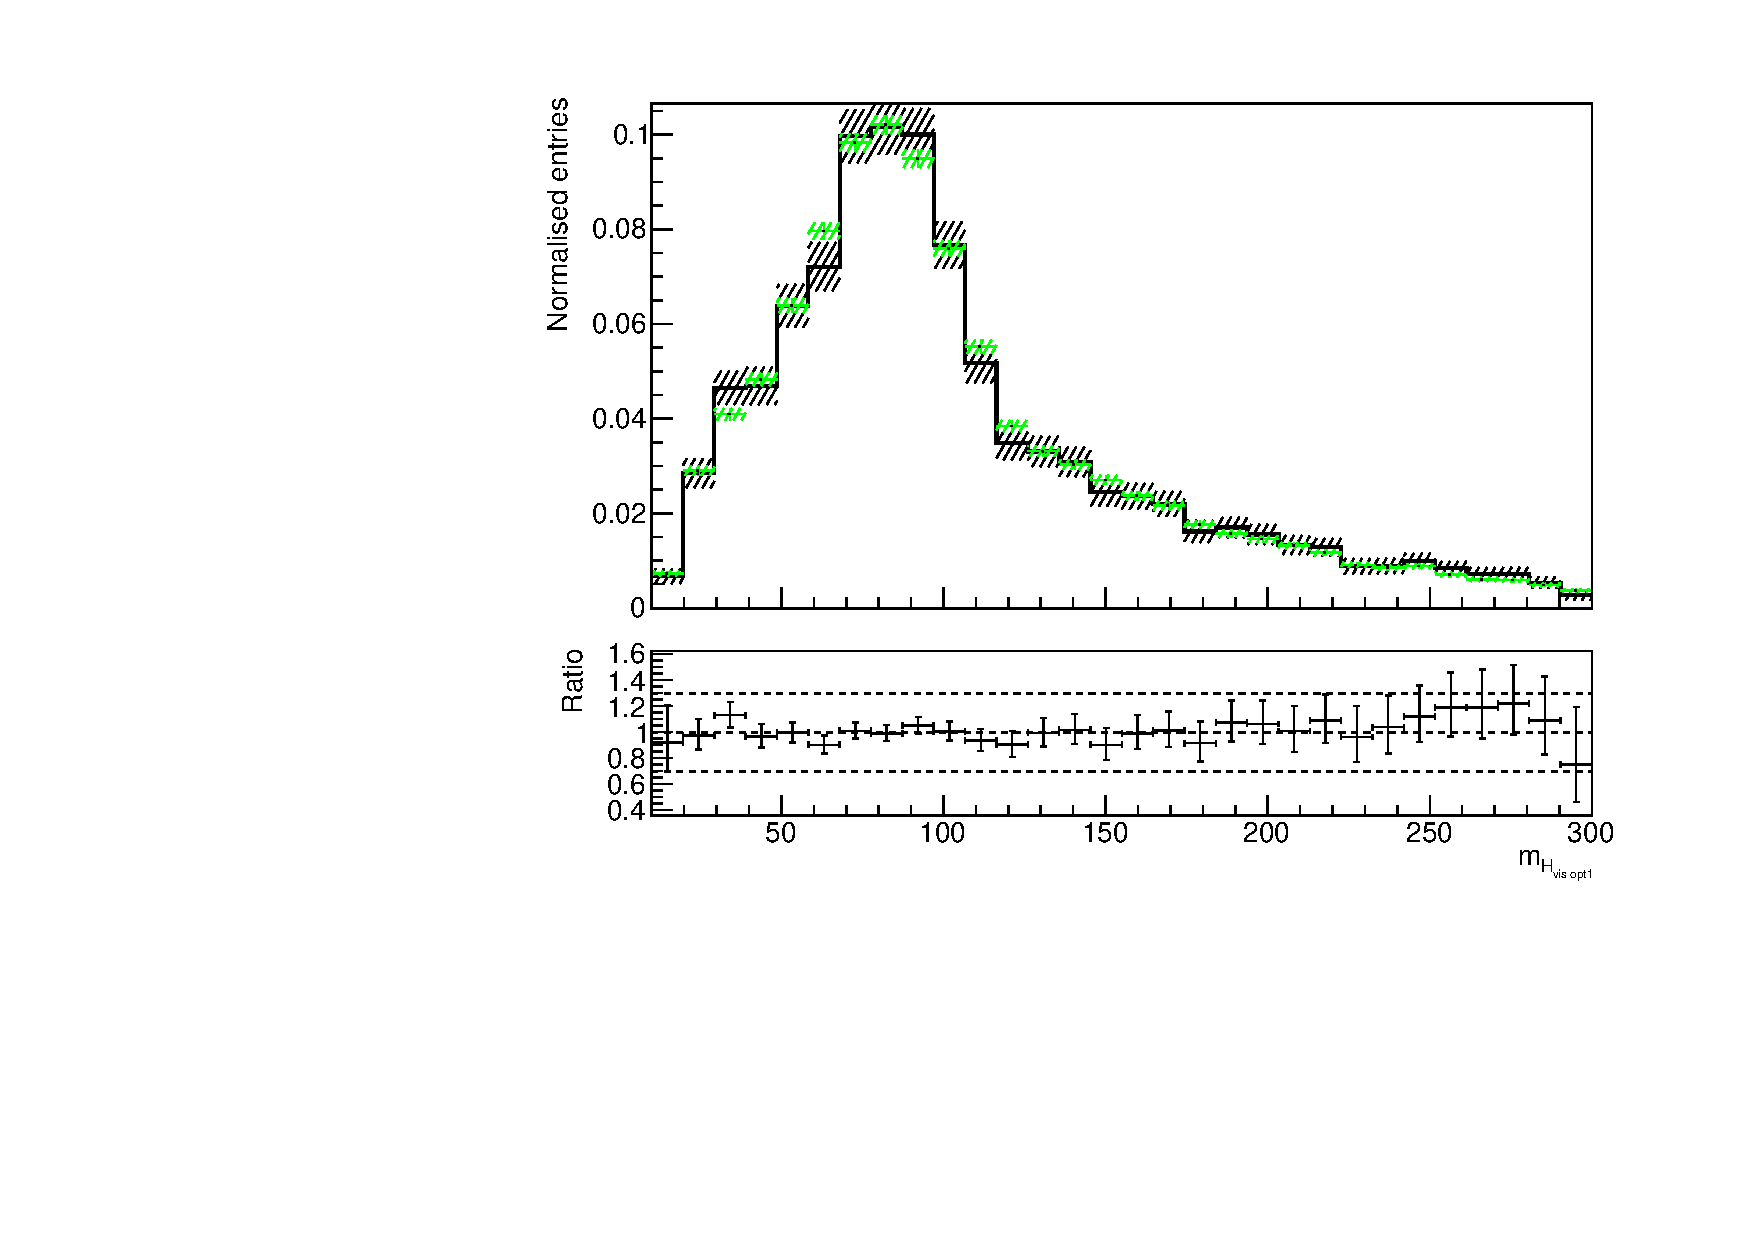
\includegraphics[width=\textwidth]{Chapter5_tHq/LeptAssociation/NegativeWeights/PosVsAll_SS_err_m_Hvis_opt1}
        \caption{$m^{\text{opt1}}_{\text{vis}}(H)$}
        \label{fig:Appendix:BDTVARS:LeptonAssignment:m_Hvis_opt1}
    \end{subfigure}
    \hfill 
    \begin{subfigure}[b]{0.44\textwidth}
        \centering
        \includegraphics[width=\textwidth]{Chapter5_tHq/LeptAssociation/NegativeWeights/PosVsAll_SS_err_deltaEta_tau_LightLep1}
        \caption{$\Delta \eta(\tauhad, \ell_{1})$}
        \label{fig:Appendix:BDTVARS:LeptonAssignmen:dEta1}
    \end{subfigure}
    
    % Second row
    \begin{subfigure}[b]{0.44\textwidth}
        \centering
        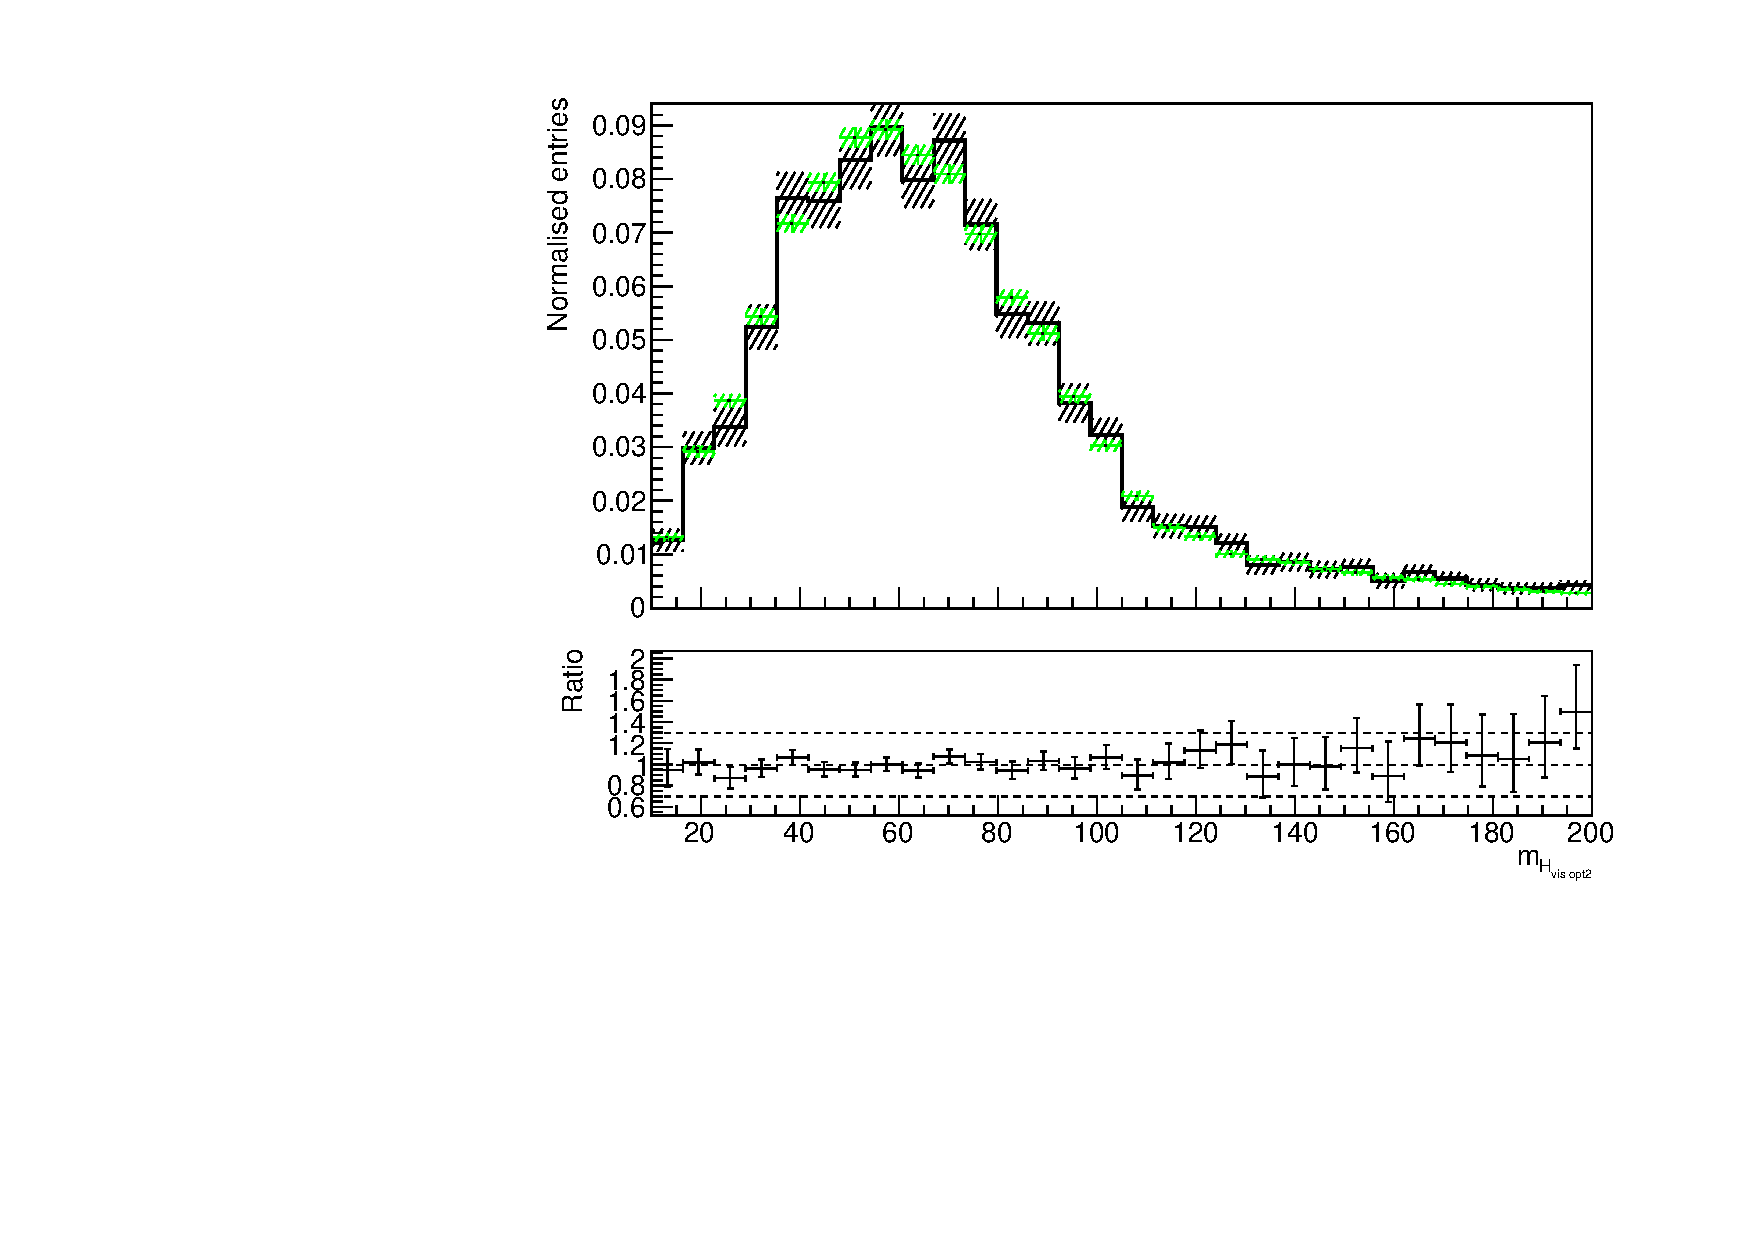
\includegraphics[width=\textwidth]{Chapter5_tHq/LeptAssociation/NegativeWeights/PosVsAll_SS_err_m_Hvis_opt2}
        \caption{$m^{\text{opt2}}_{\text{vis}}(\PHiggs)$}
        \label{fig:Appendix:BDTVARS:LeptonAssignmen:m_H2}
    \end{subfigure}
    \hfill
    \begin{subfigure}[b]{0.44\textwidth}
        \centering
        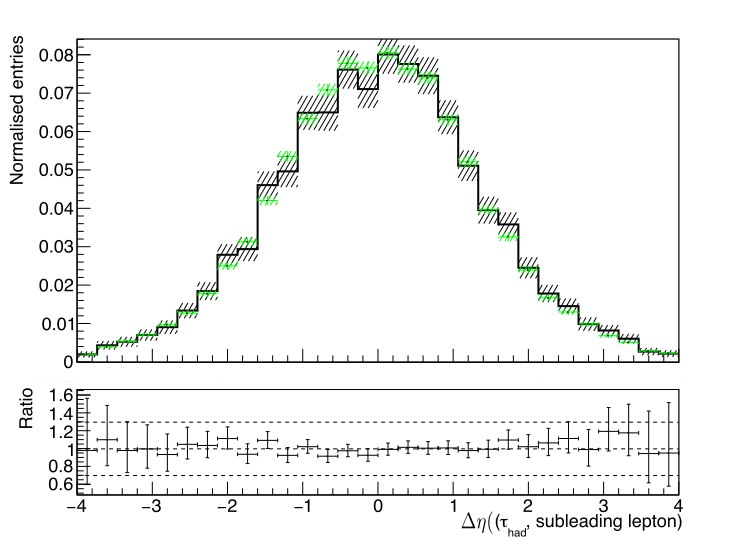
\includegraphics[width=\textwidth]{Chapter5_tHq/LeptAssociation/NegativeWeights/PosVsAll_SS_err_deltaEta_tau_LightLep2_fixed}
        \caption{$\Delta \eta(\tauhad, \ell_{2})$}
        \label{fig:Appendix:BDTVARS:LeptonAssignmen:dEta2}
    \end{subfigure}
    \caption{Normalised distributions of the highest ranked variables for the light-lepton assignment. 
    The black distribution is obtained using all events and the green one corresponds to the escenario in
    which only the positively weighted events are used. The comparison between the Type$\,$1 and Type$\,$2
    categories for these variables is presented on
    Figure~\ref{fig:ChaptH:LepAsign:SS:BDT:inputFeatuerRanked}.}
    \label{fig:Appendix:BDTVARS:LeptonAssignmen:Top$}
\end{figure}



\begin{comment}
%% 1
\begin{figure}[h]
\centering
\begin{subfigure}{.45\textwidth}
  \centering
  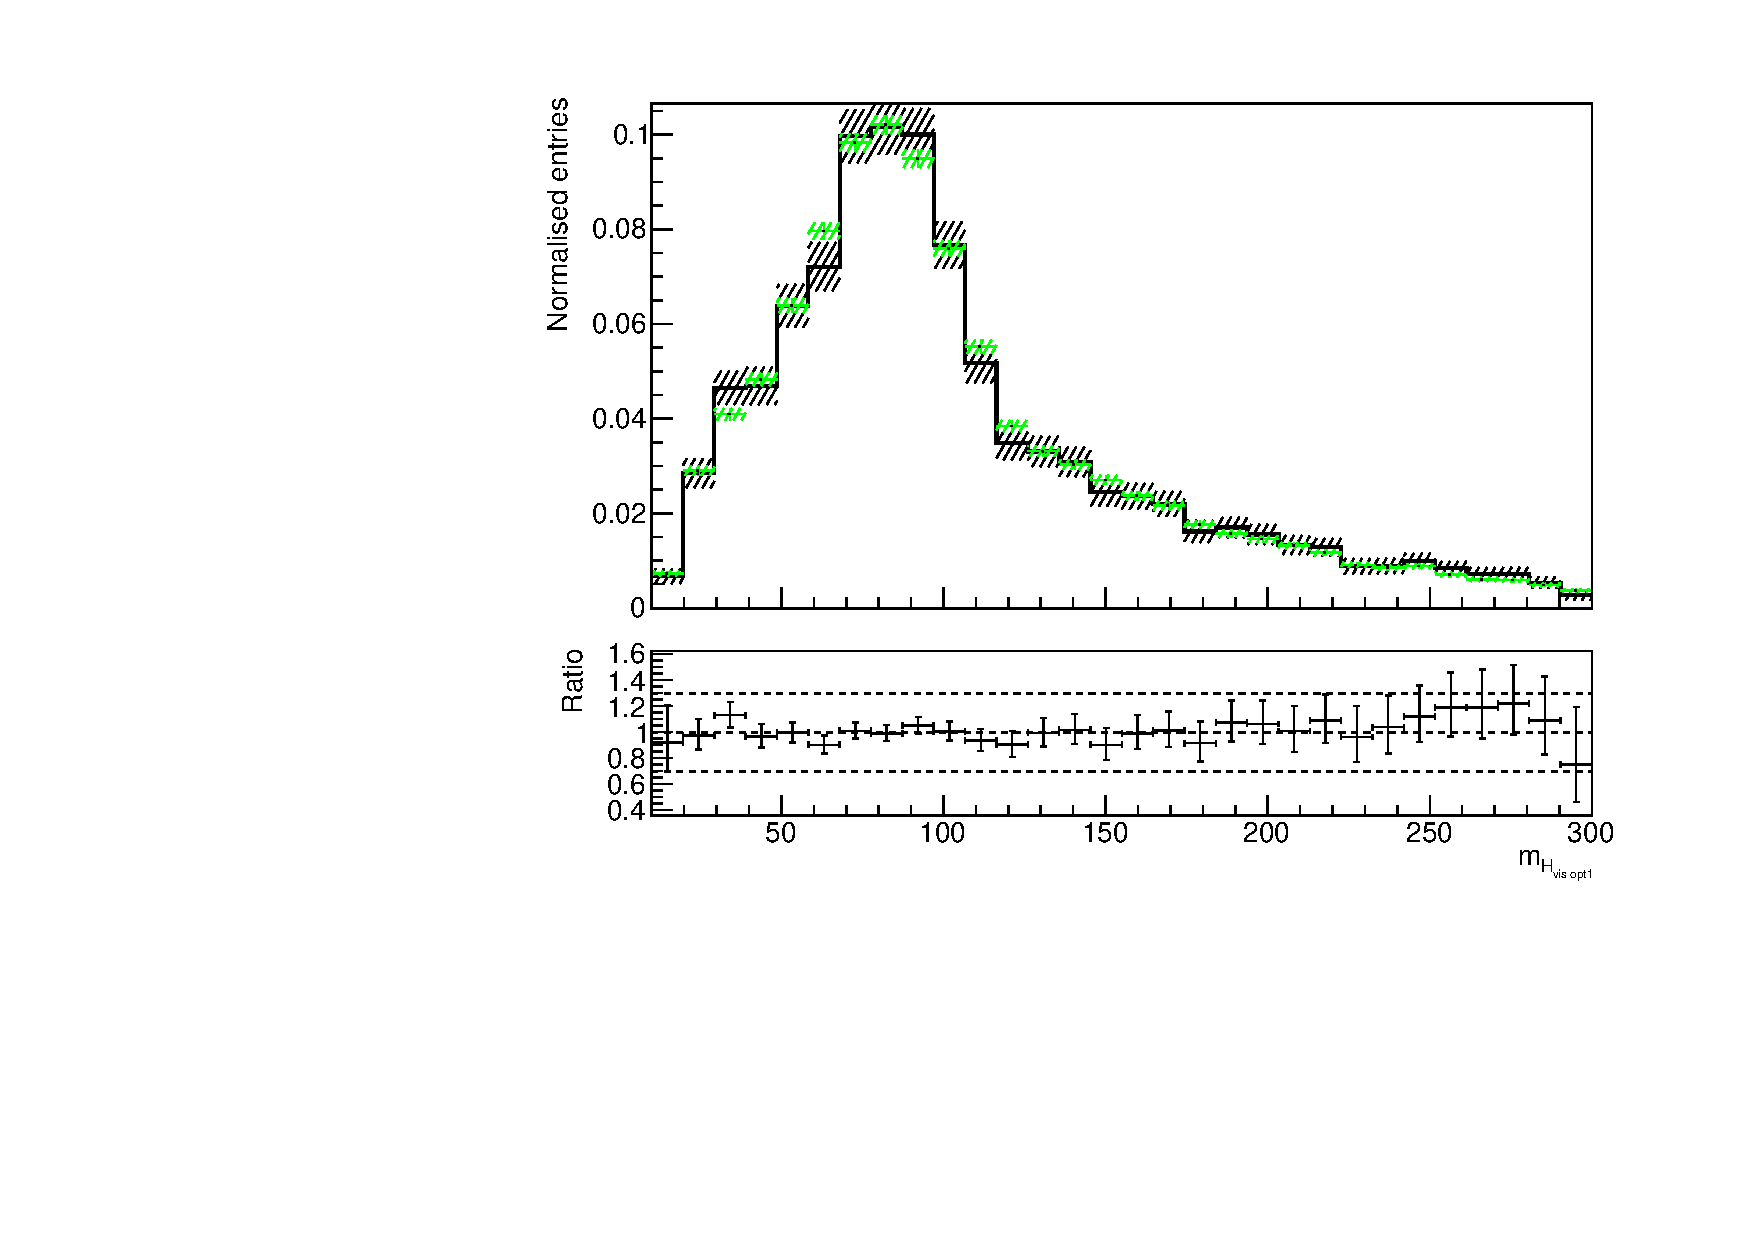
\includegraphics[width=.95\linewidth]{Chapter5_tHq/LeptAssociation/NegativeWeights/PosVsAll_SS_err_m_Hvis_opt1}
  %\caption{}
\end{subfigure}%
\begin{subfigure}{.46\textwidth}
  \centering
  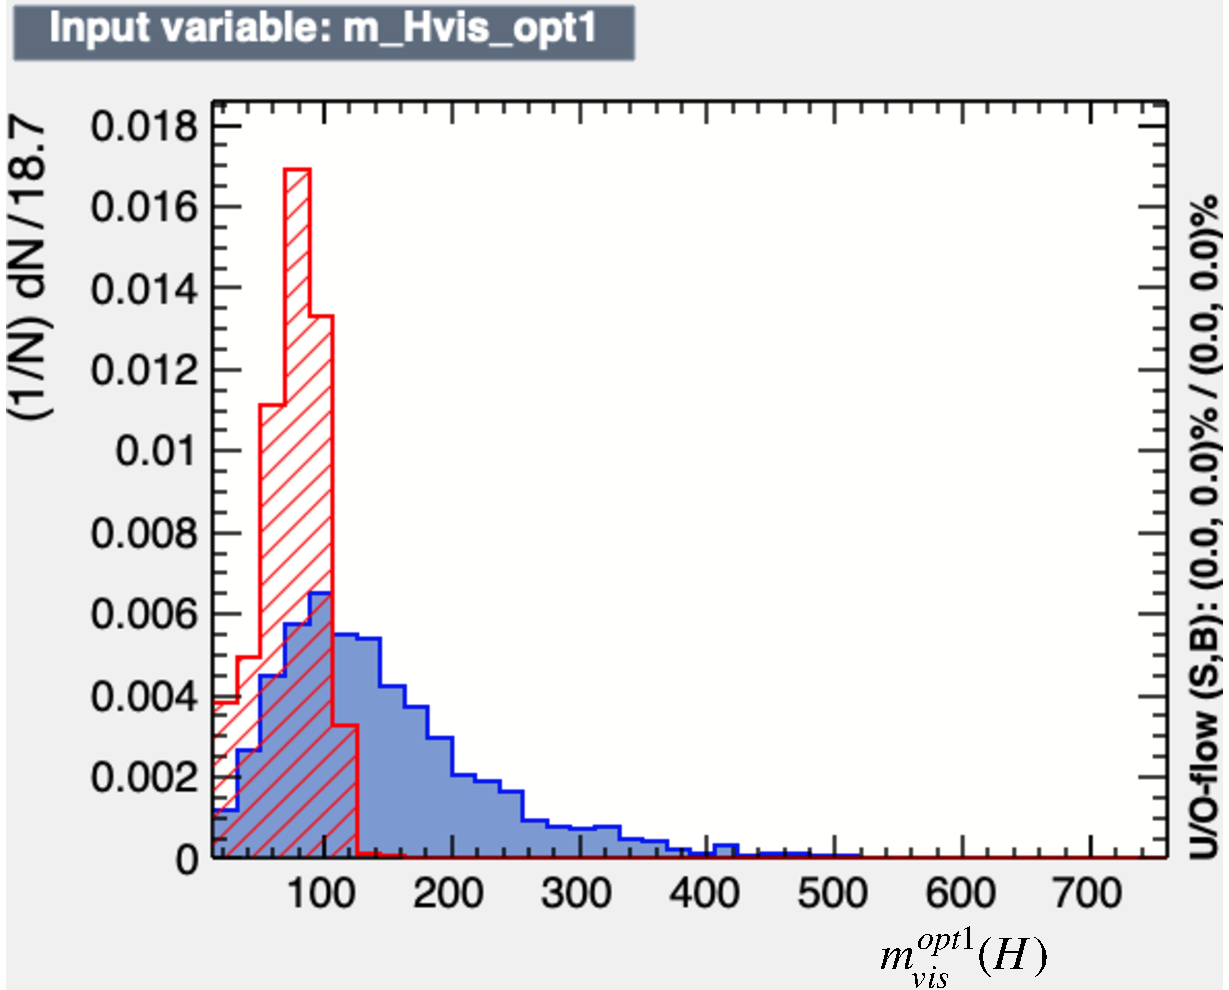
\includegraphics[width=.95\linewidth]{Chapter5_tHq/LeptAssociation/BDT_InputVariables/pdf_input_m_Hvis_opt1}
  %\caption{}
\end{subfigure}
\caption{Normalised distributions for $m^{\text{opt1}}_{\text{vis}}(H)$.}
\label{fig:Appendix:BDTVARS:LeptonAssignment:m_Hvis_opt1}
\end{figure}

%% 2
\begin{figure}[h]
\centering
\begin{subfigure}{.46\textwidth}
  \centering
  \includegraphics[width=.95\linewidth]{Chapter5_tHq/LeptAssociation/NegativeWeights/PosVsAll_SS_err_deltaEta_tau_LightLep1}
  %\caption{}
\end{subfigure}%
\begin{subfigure}{.46\textwidth}
  \centering
  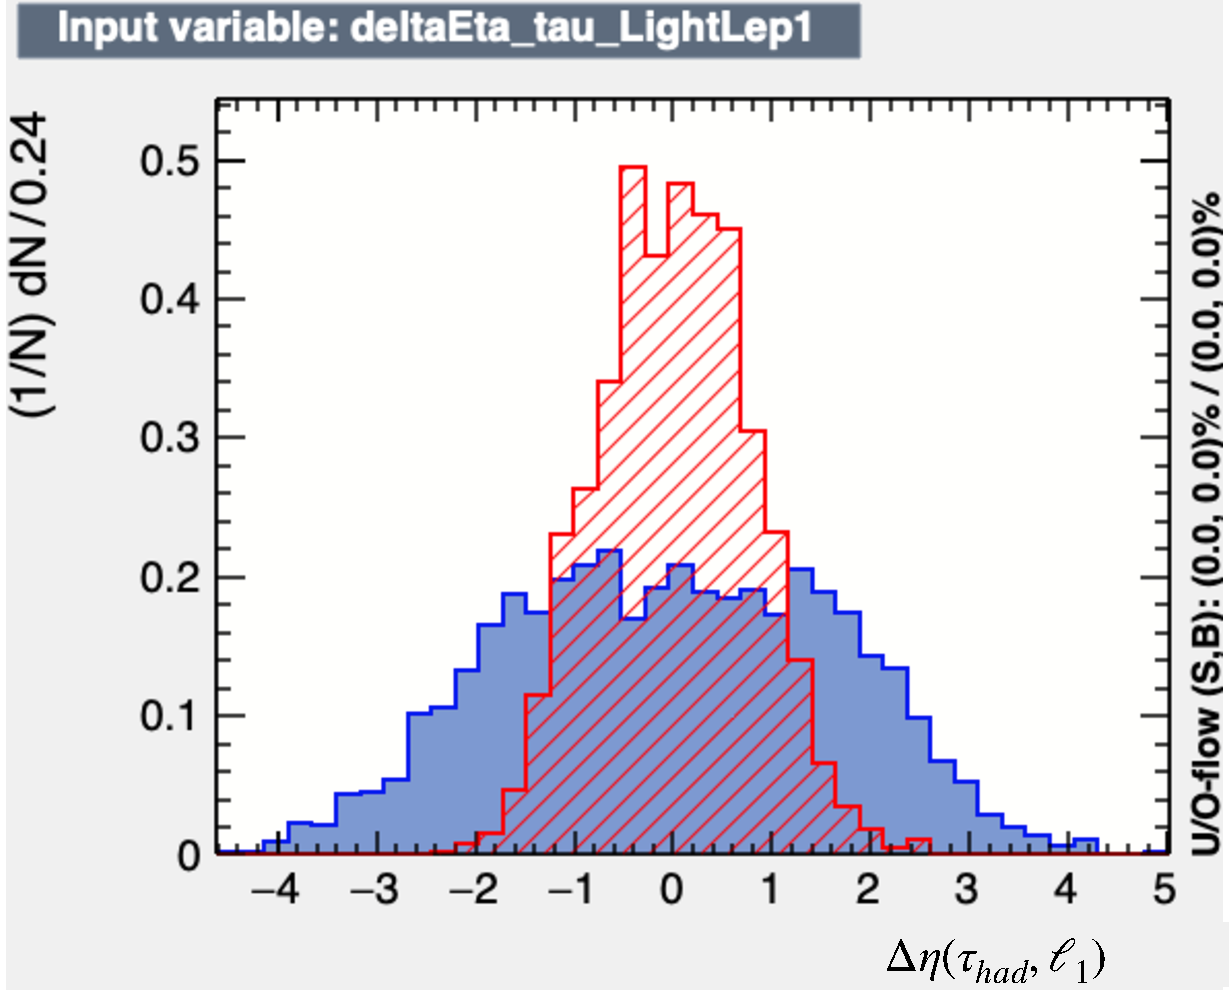
\includegraphics[width=.95\linewidth]{Chapter5_tHq/LeptAssociation/BDT_InputVariables/pdf_input_deltaEta_tau_LightLep1}
  %\caption{}
\end{subfigure}
\caption{Normalised distributions for $\Delta \eta(\tauhad, \ell_{1})$.}
\label{fig:Appendix:BDTVARS:LeptonAssignment:deltaEta_tau_LightLep1}
\end{figure}

%% 3
\begin{figure}[h]
\centering
\begin{subfigure}{.46\textwidth}
  \centering
  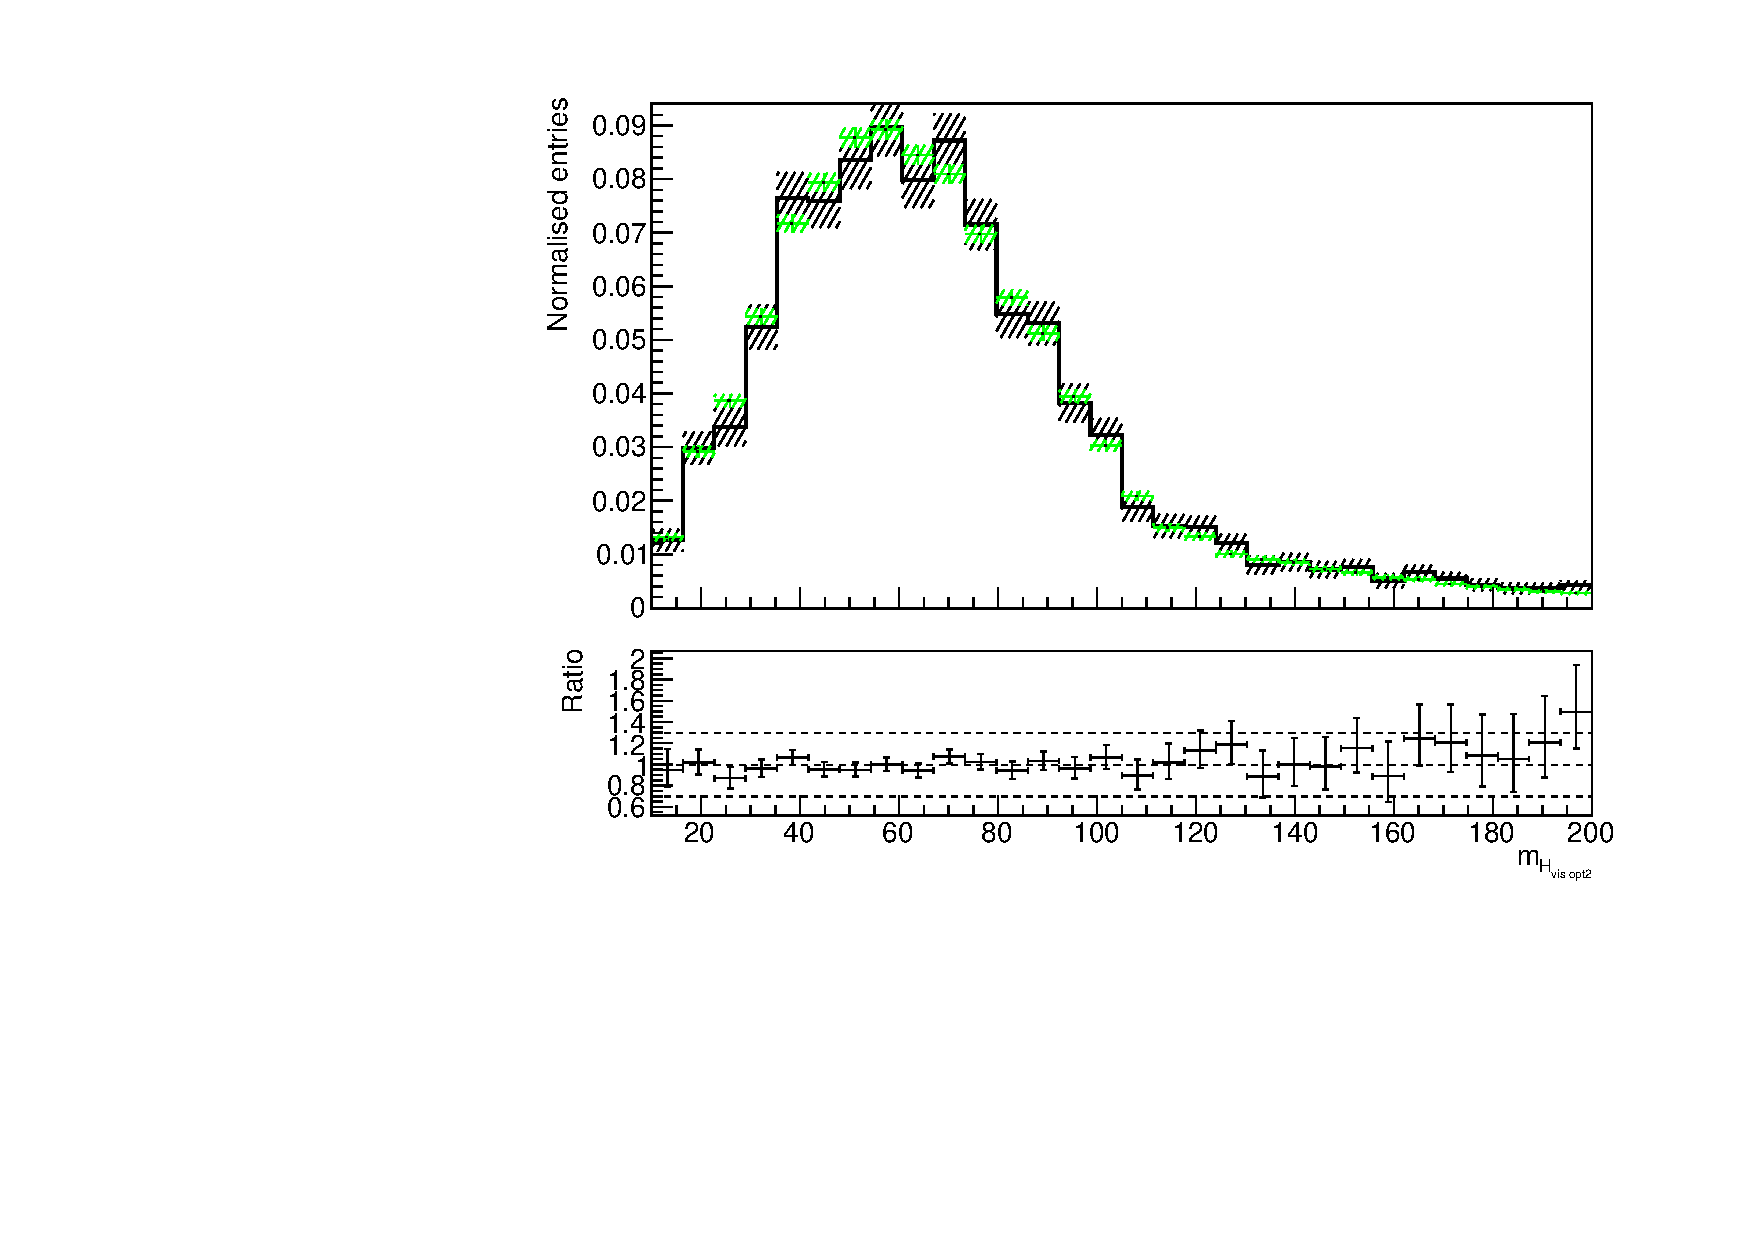
\includegraphics[width=.95\linewidth]{Chapter5_tHq/LeptAssociation/NegativeWeights/PosVsAll_SS_err_m_Hvis_opt2}
  %\caption{}
\end{subfigure}%
\begin{subfigure}{.46\textwidth}
  \centering
  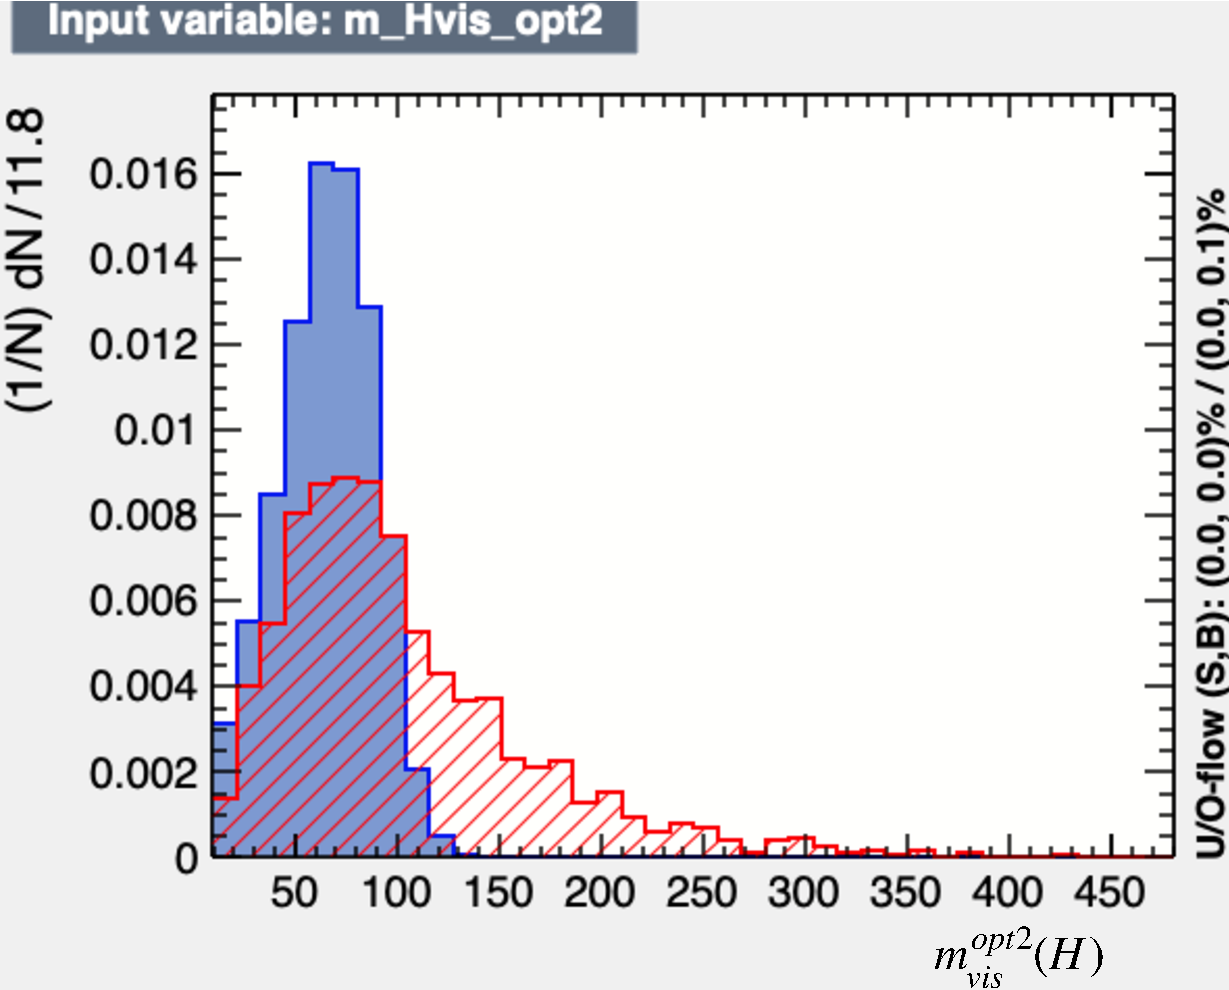
\includegraphics[width=.95\linewidth]{Chapter5_tHq/LeptAssociation/BDT_InputVariables/pdf_input_m_Hvis_opt2}
  %\caption{}
\end{subfigure}
\caption{Normalised distributions for $m^{\text{opt2}}_{\text{vis}}(\PHiggs)$.}
\label{fig:Appendix:BDTVARS:LeptonAssignment:m_Hvis_opt2}
\end{figure}

%% 4
\begin{figure}[h]
\centering
\begin{subfigure}{.46\textwidth}
  \centering
  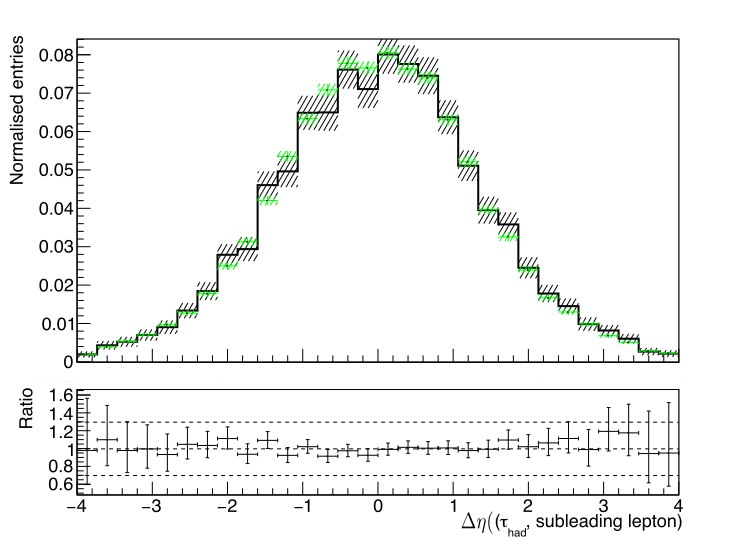
\includegraphics[width=.95\linewidth]{Chapter5_tHq/LeptAssociation/NegativeWeights/PosVsAll_SS_err_deltaEta_tau_LightLep2_fixed}
  %\caption{}
\end{subfigure}%
\begin{subfigure}{.46\textwidth}
  \centering
  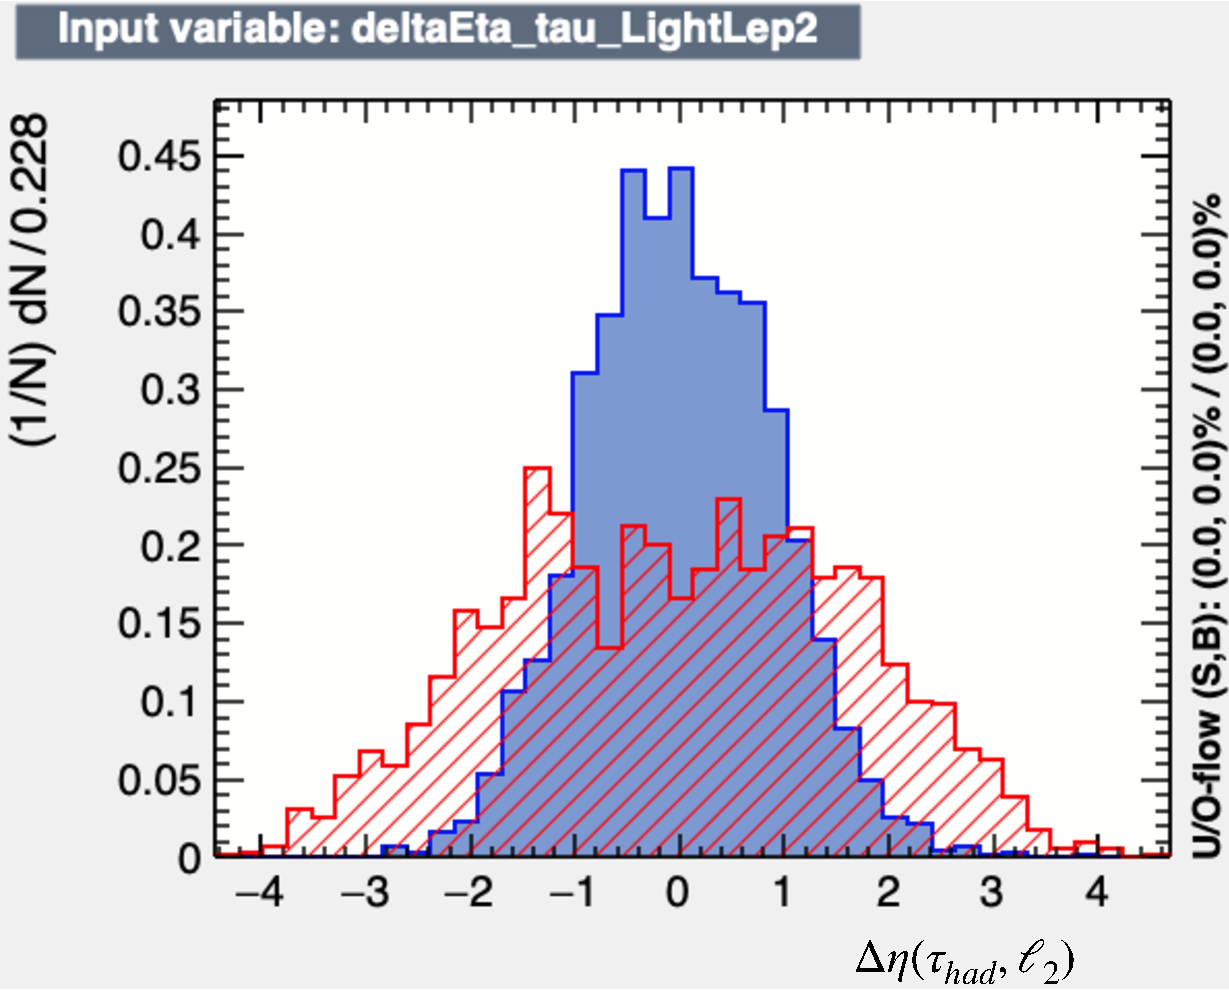
\includegraphics[width=.95\linewidth]{Chapter5_tHq/LeptAssociation/BDT_InputVariables/pdf_input_deltaEta_tau_LightLep2}
  %\caption{}
\end{subfigure}
\caption{Normalised distributions for $\Delta \eta(\tauhad, \ell_{2})$.}
\label{fig:Appendix:BDTVARS:LeptonAssignment:deltaEta_tau_LightLep2}
\end{figure}
\end{comment}

%% 5
\begin{figure}[h]
\centering
\begin{subfigure}{.46\textwidth}
  \centering
  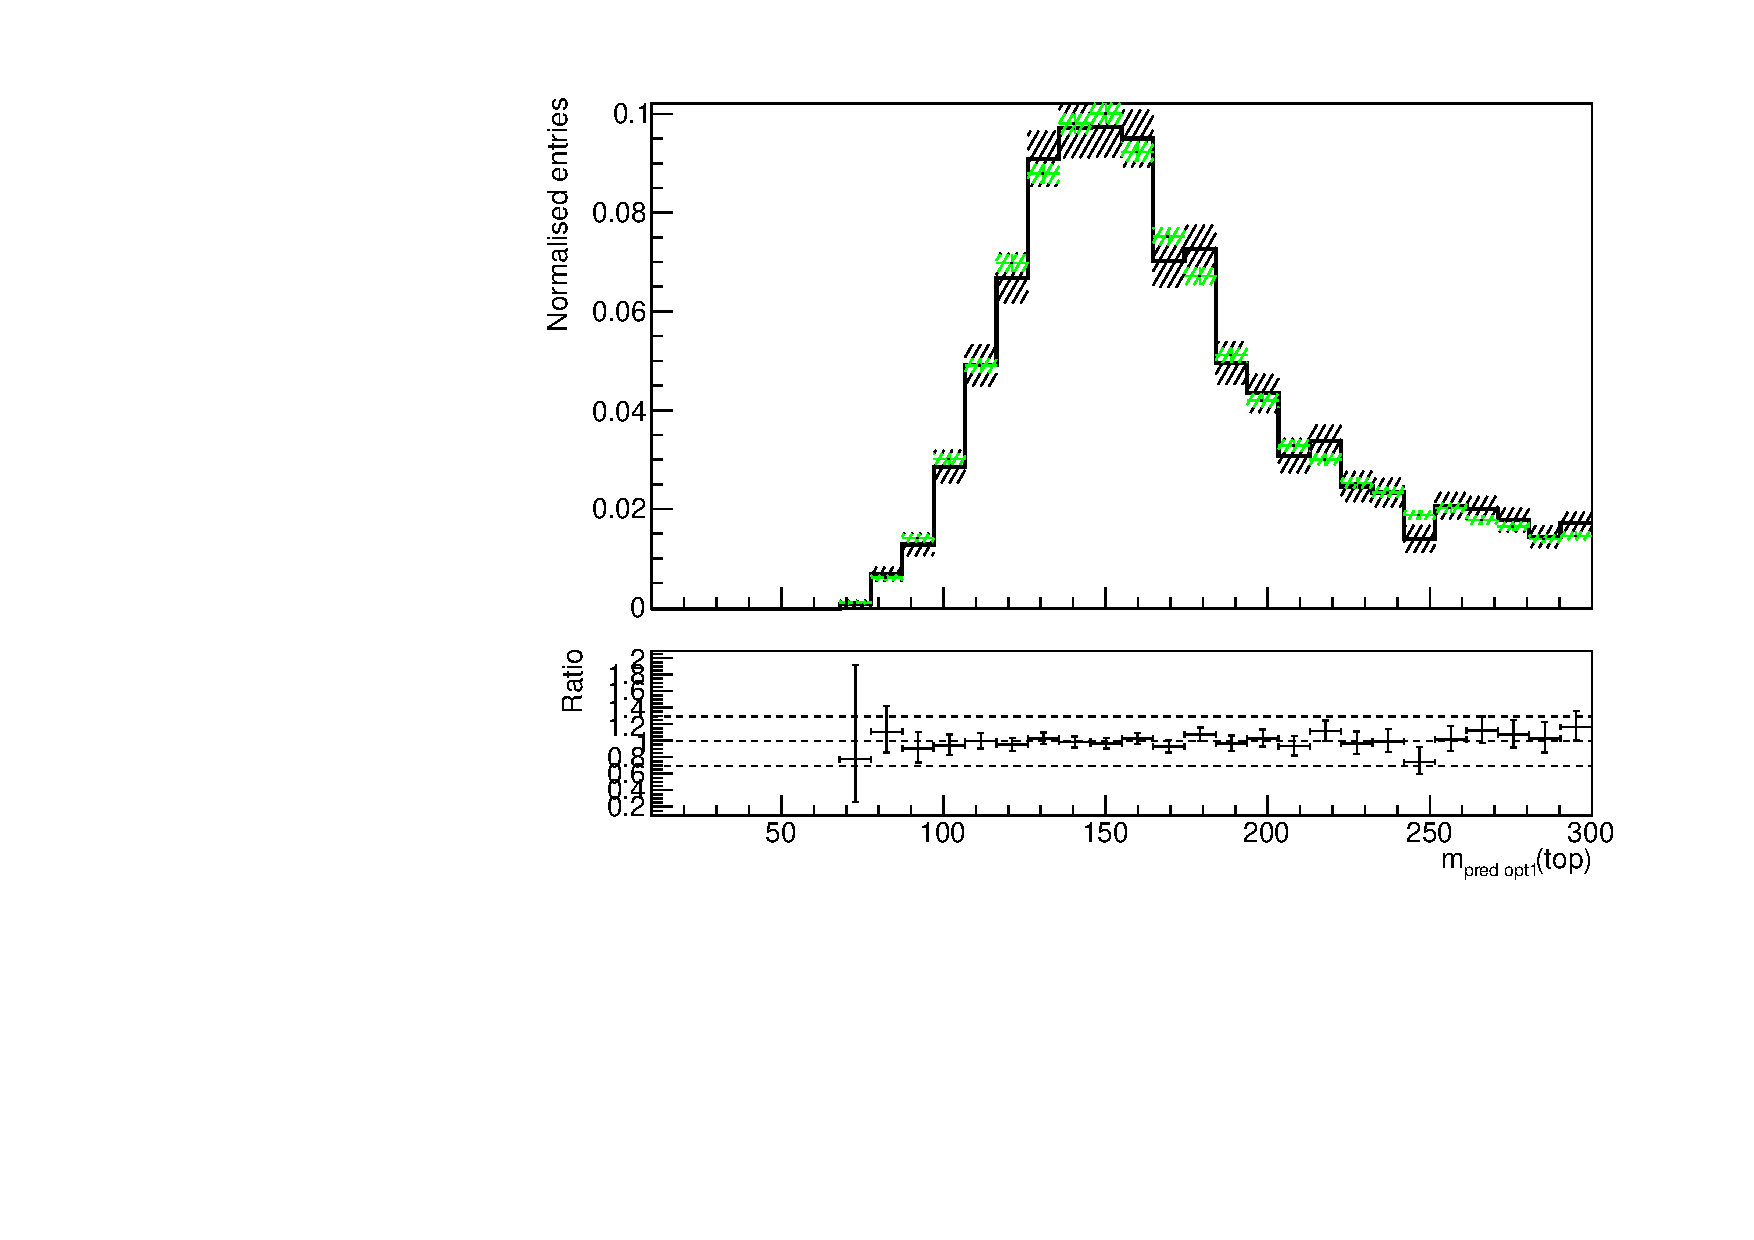
\includegraphics[width=.95\linewidth]{Chapter5_tHq/LeptAssociation/NegativeWeights/PosVsAll_SS_err_m_Tpred_opt1}
  %\caption{}
\end{subfigure}%
\begin{subfigure}{.46\textwidth}
  \centering
  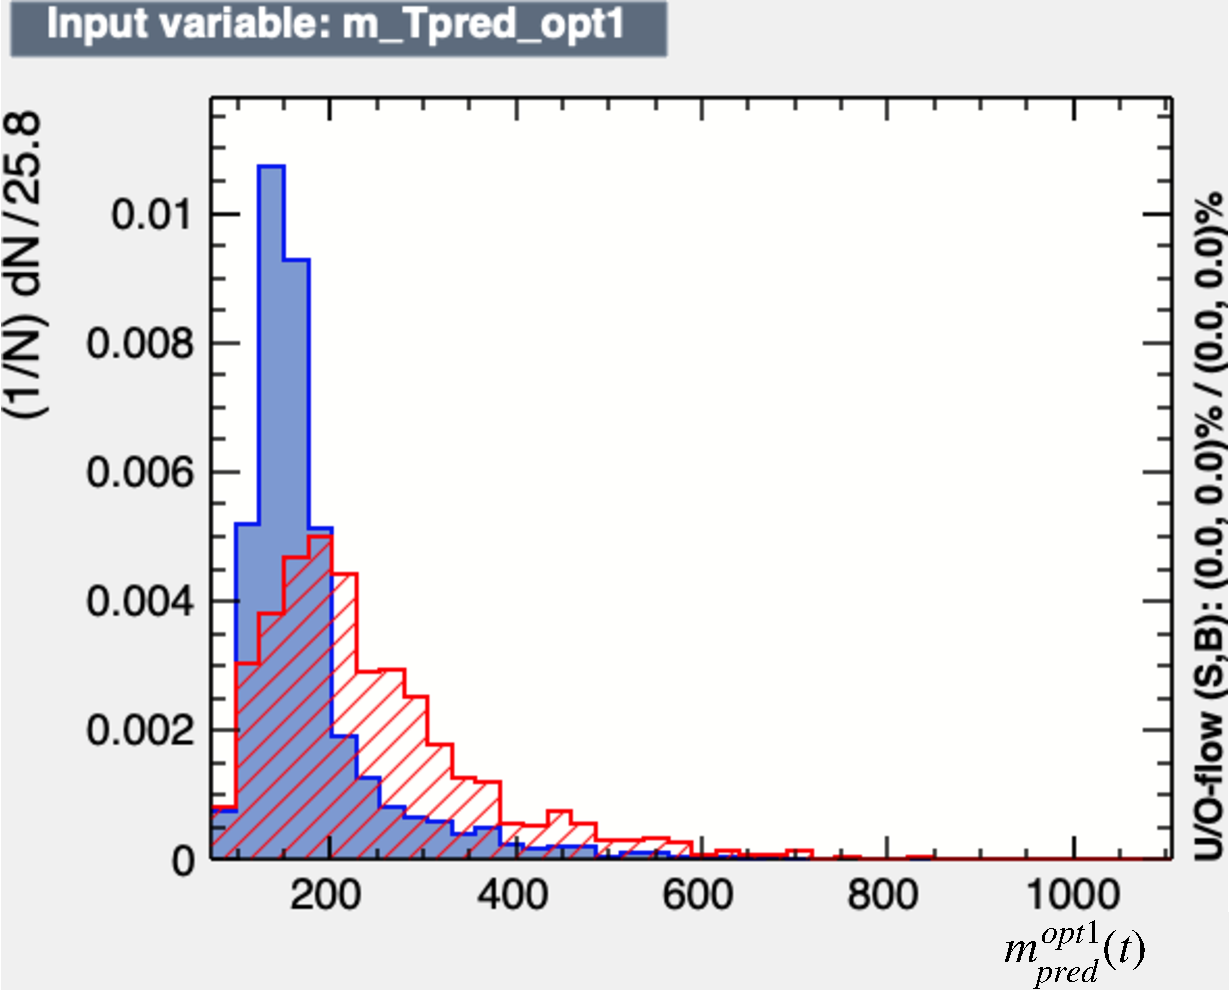
\includegraphics[width=.95\linewidth]{Chapter5_tHq/LeptAssociation/BDT_InputVariables/pdf_input_m_Tpred_opt1}
  %\caption{}
\end{subfigure}
\caption{Normalised distributions for $m^{\text{opt1}}_{\text{pred}}(t)$.}
\label{fig:Appendix:BDTVARS:LeptonAssignment:m_Tpred_opt1}
\end{figure}

%% 6
\begin{figure}[h]
\centering
\begin{subfigure}{.46\textwidth}
  \centering
  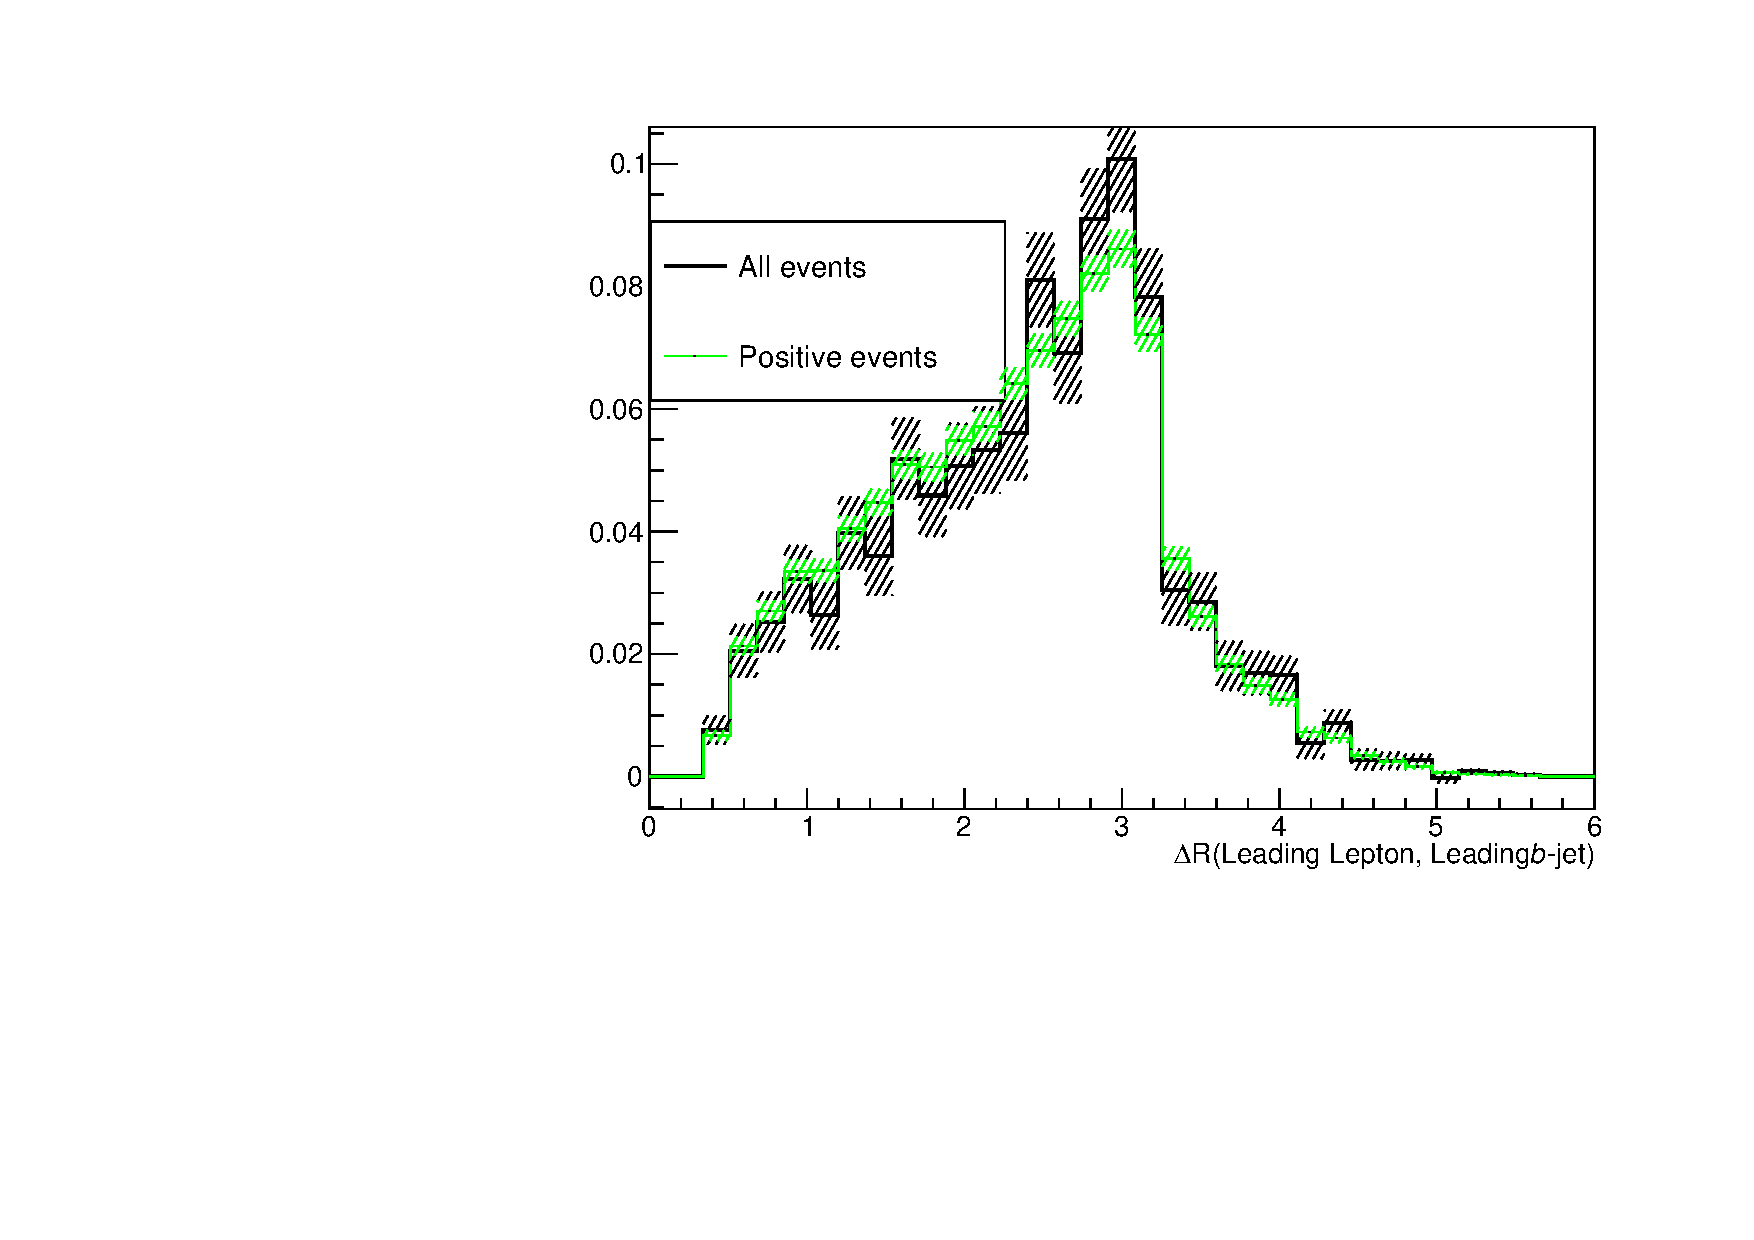
\includegraphics[width=.95\linewidth]{Chapter5_tHq/LeptAssociation/NegativeWeights/PosVsAll_SS_err_deltaR_b_LightLep1}
  %\caption{}
\end{subfigure}%
\begin{subfigure}{.46\textwidth}
  \centering
  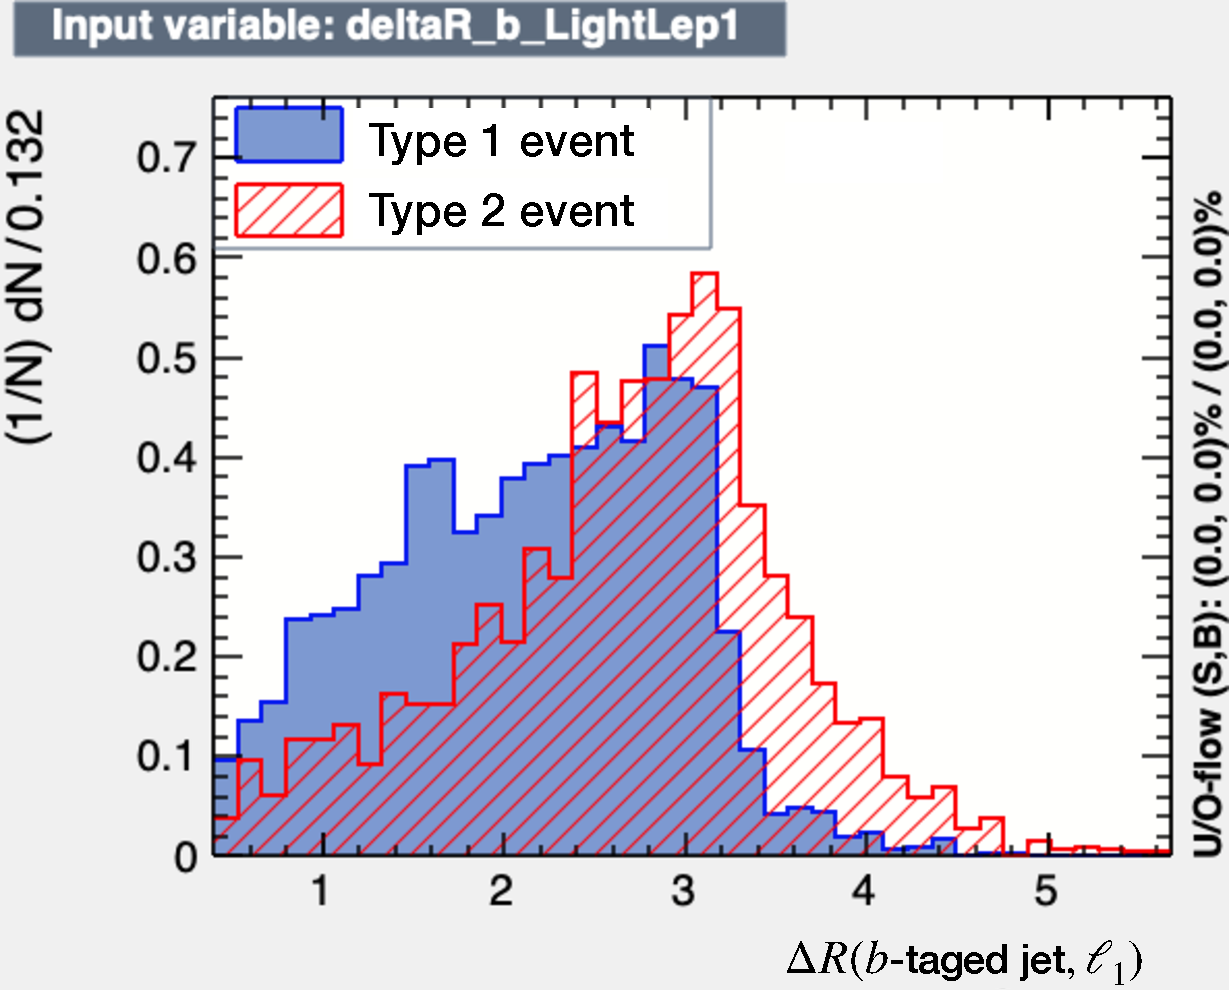
\includegraphics[width=.95\linewidth]{Chapter5_tHq/LeptAssociation/BDT_InputVariables/pdf_input_deltaR_b_LightLep1}
  %\caption{}
\end{subfigure}
\caption{Normalised distributions for the geometric proximity, $\Delta R$, between the \btagged jet and the leading-light lepton.}
\label{fig:Appendix:BDTVARS:LeptonAssignment:deltaR_b_LightLep1}
\end{figure}

%% 7
\begin{figure}[h]
\centering
\begin{subfigure}{.46\textwidth}
  \centering
  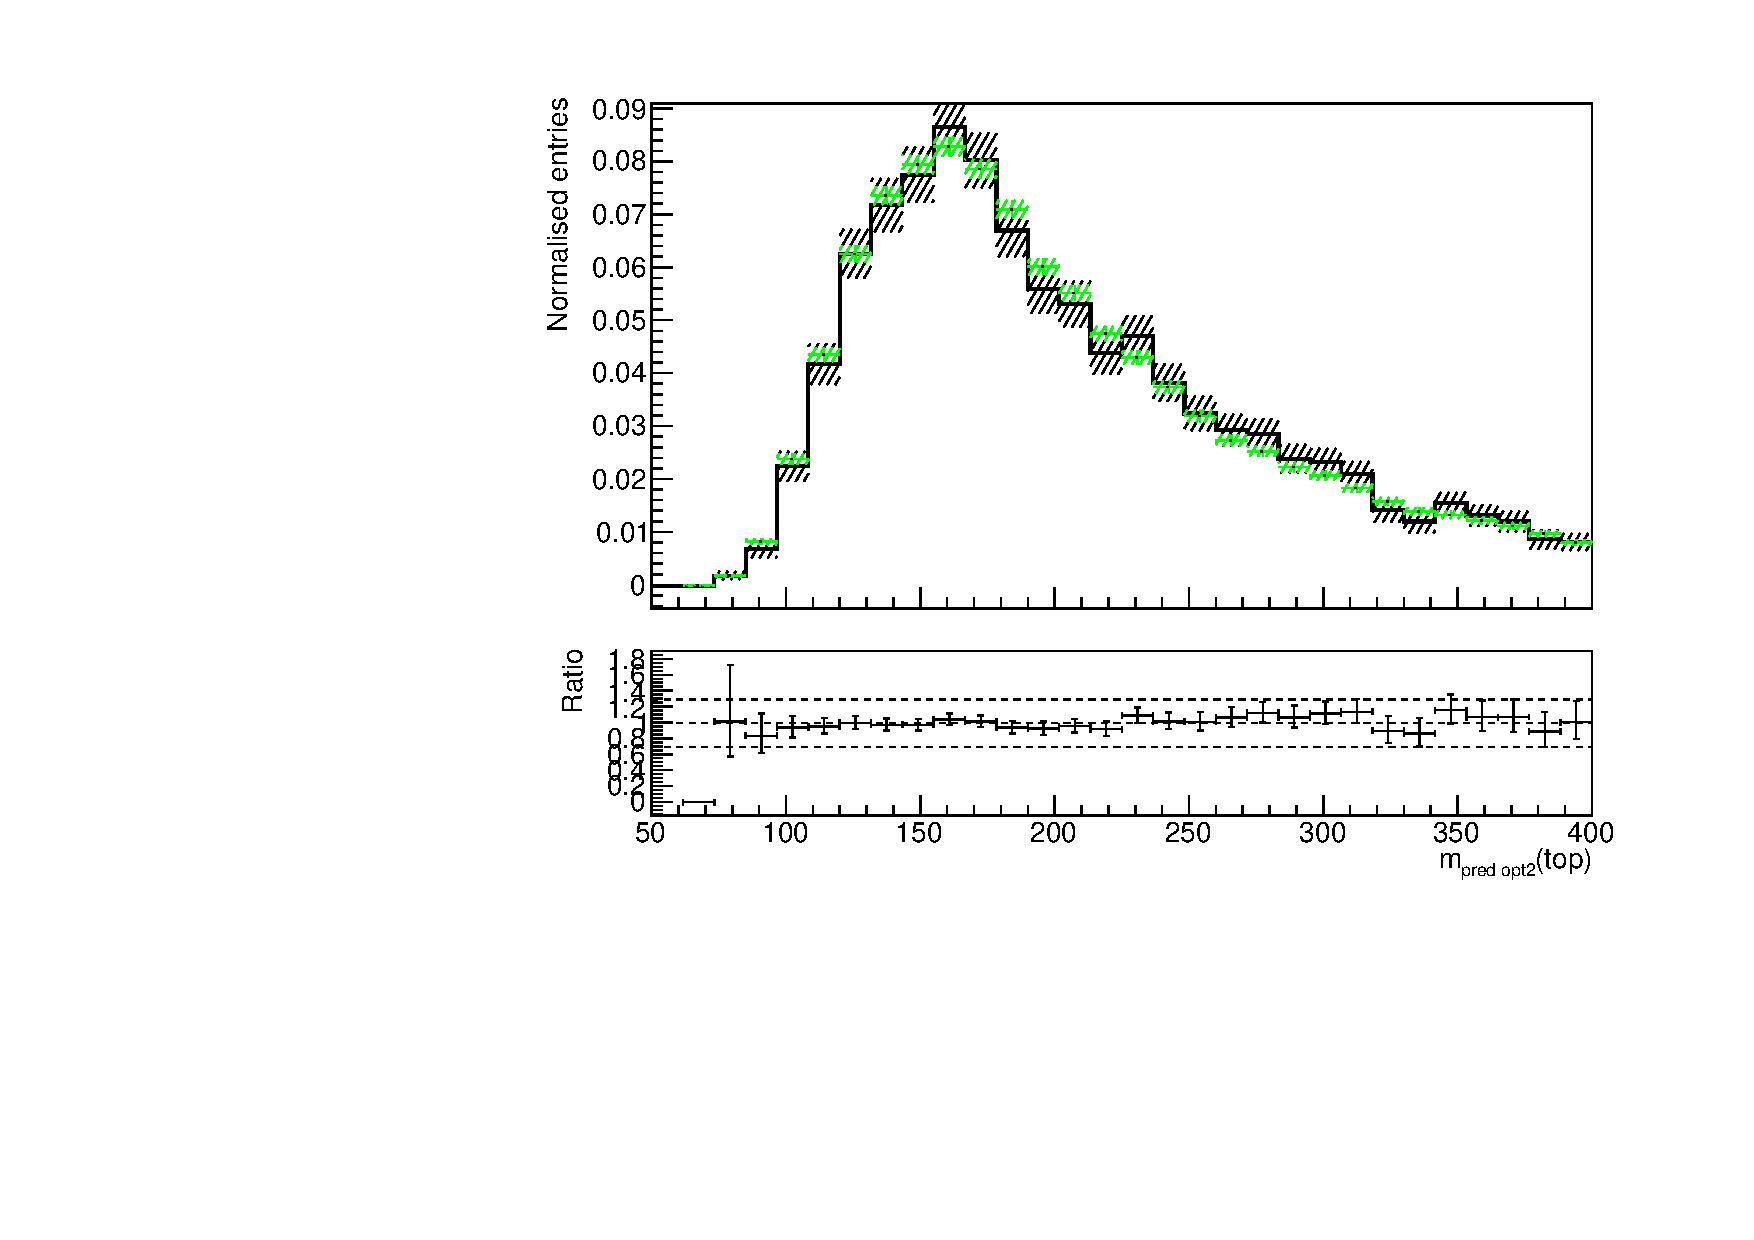
\includegraphics[width=.95\linewidth]{Chapter5_tHq/LeptAssociation/NegativeWeights/PosVsAll_SS_err_m_Tpred_opt2}
  %\caption{}
\end{subfigure}%
\begin{subfigure}{.46\textwidth}
  \centering
  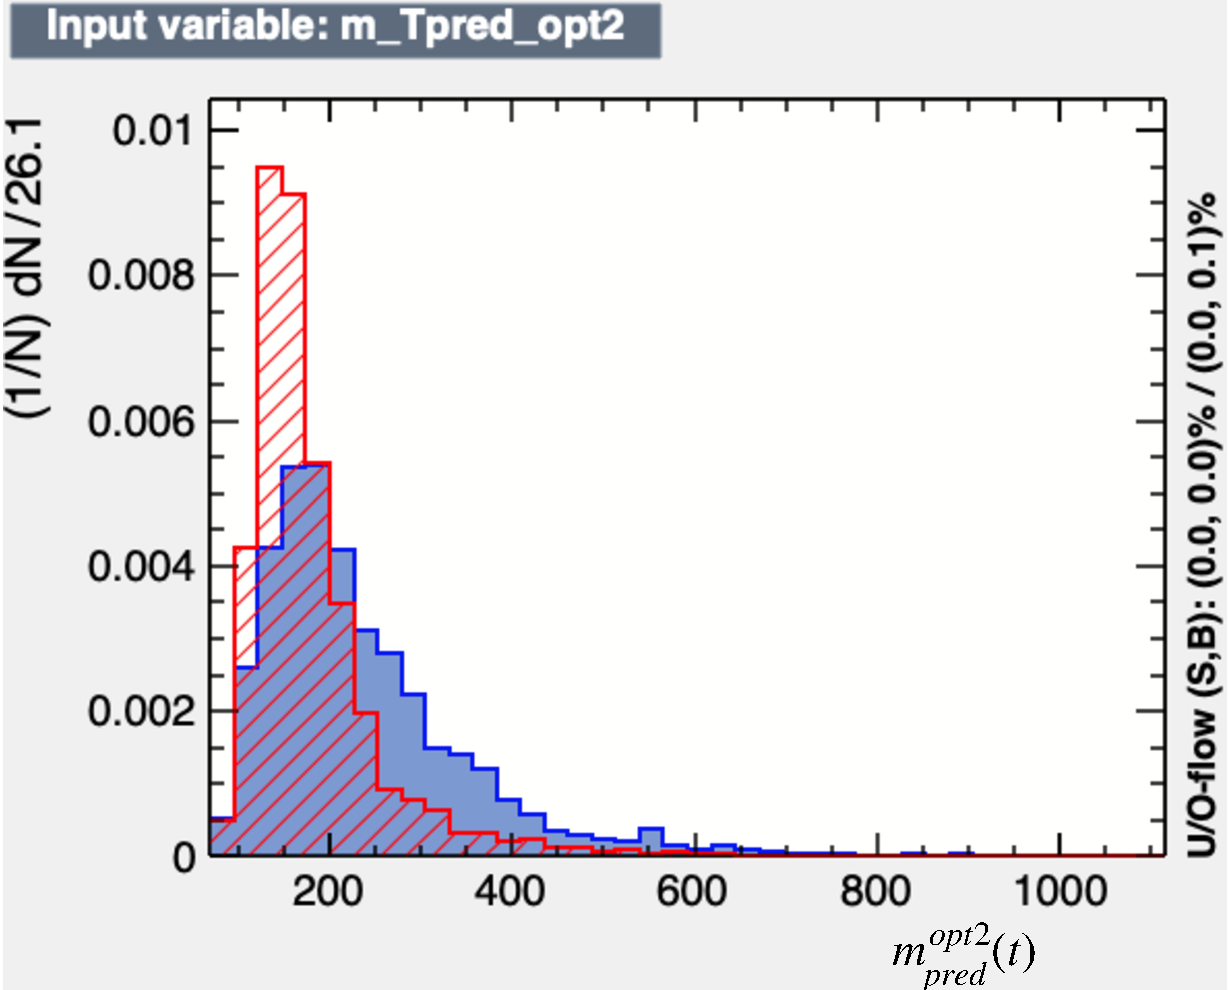
\includegraphics[width=.95\linewidth]{Chapter5_tHq/LeptAssociation/BDT_InputVariables/pdf_input_m_Tpred_opt2}
  %\caption{}
\end{subfigure}
\caption{Normalised distributions for $m^{\text{opt2}}_{\text{pred}}(t)$.}
\label{fig:Appendix:BDTVARS:LeptonAssignment:m_Tpred_opt2}
\end{figure}

%% 8
\begin{figure}[h]
\centering
\begin{subfigure}{.46\textwidth}
  \centering
  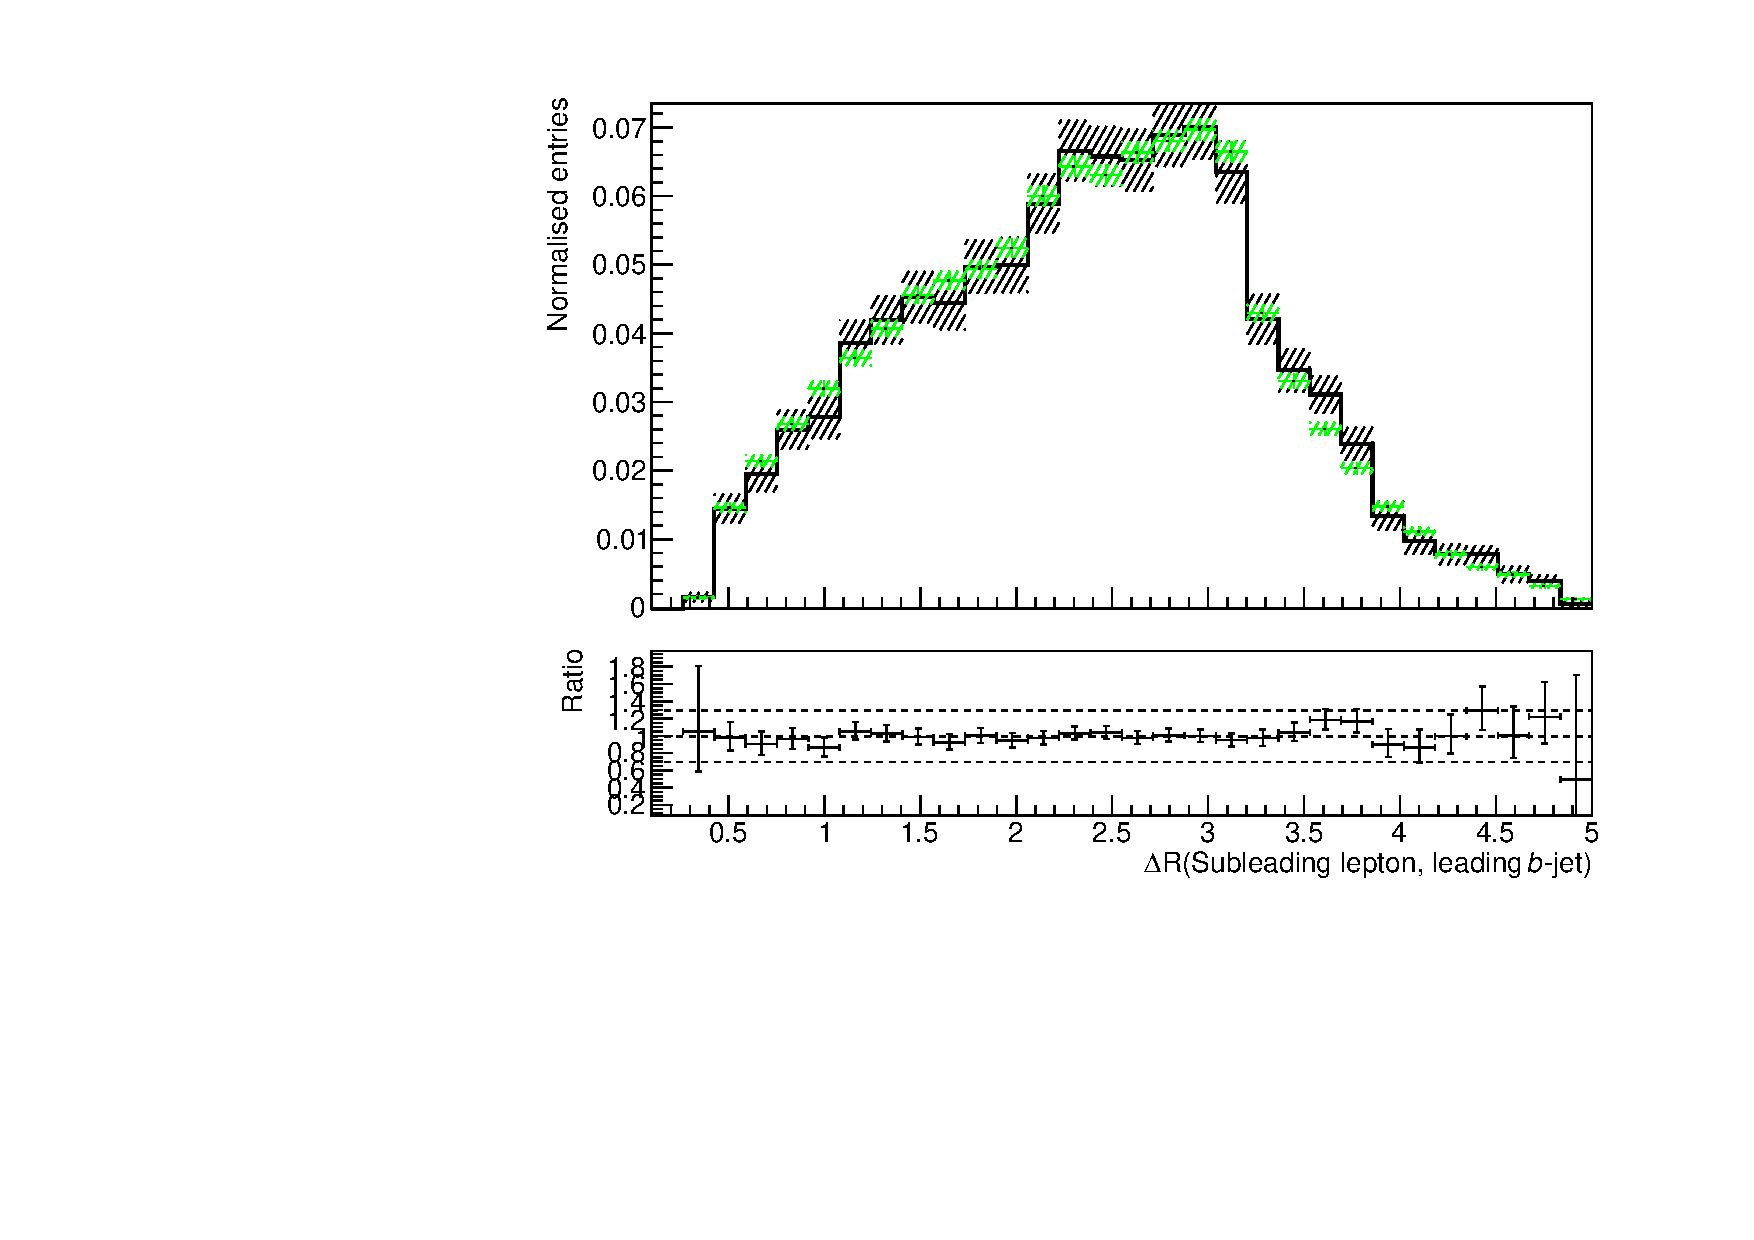
\includegraphics[width=.95\linewidth]{Chapter5_tHq/LeptAssociation/NegativeWeights/PosVsAll_SS_err_deltaR_b_LightLep2}
  %\caption{}
\end{subfigure}%
\begin{subfigure}{.46\textwidth}
  \centering
  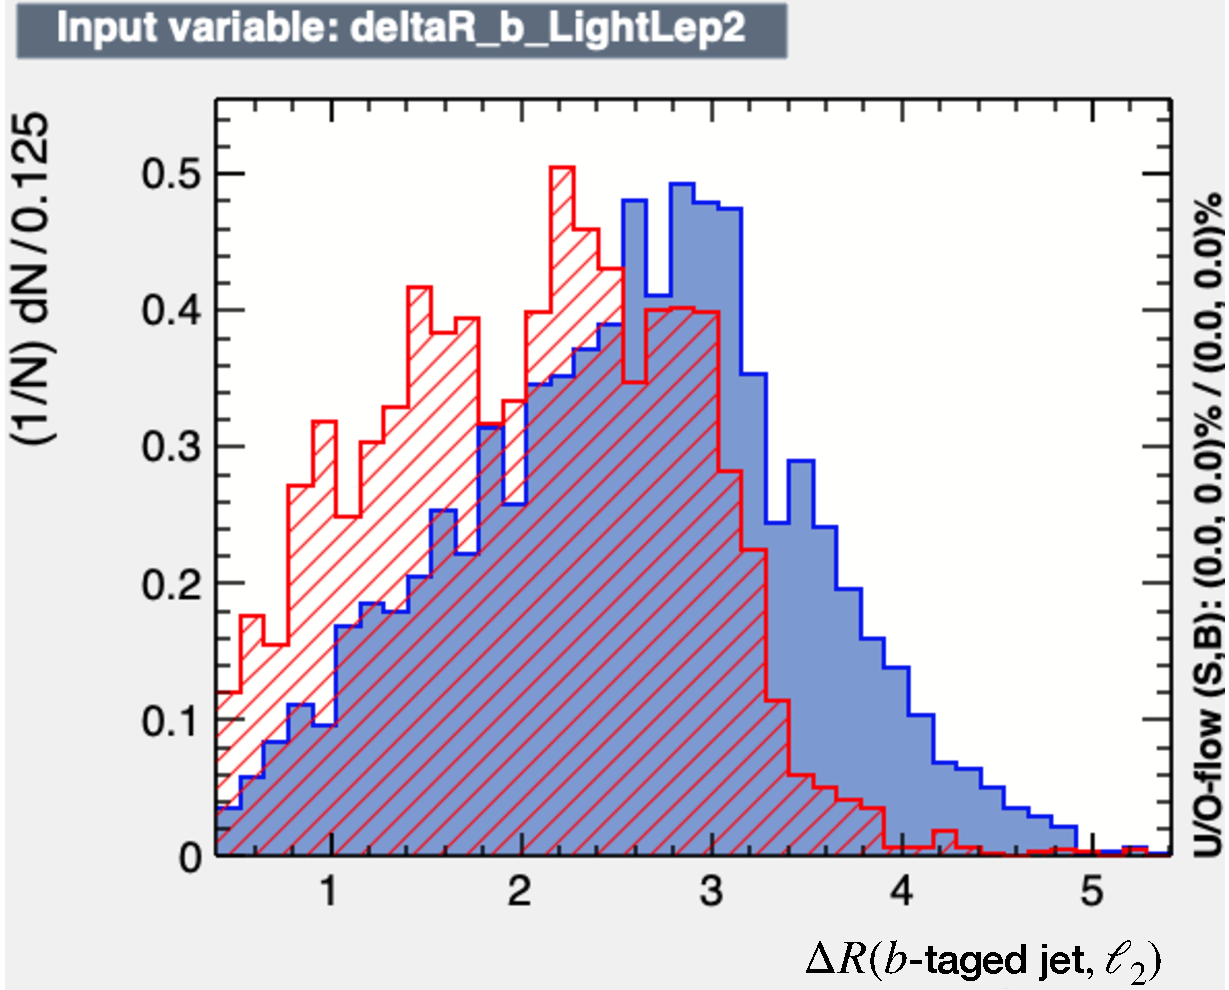
\includegraphics[width=.95\linewidth]{Chapter5_tHq/LeptAssociation/BDT_InputVariables/pdf_input_deltaR_b_LightLep2}
  %\caption{}
\end{subfigure}
\caption{Normalised distributions for $\Delta R(b\text{-taged jet}, \ell_{2})$.}
\label{fig:Appendix:BDTVARS:LeptonAssignment:deltaR_b_LightLep2}
\end{figure}

%% 9
\begin{figure}[h]
\centering
\begin{subfigure}{.46\textwidth}
  \centering
  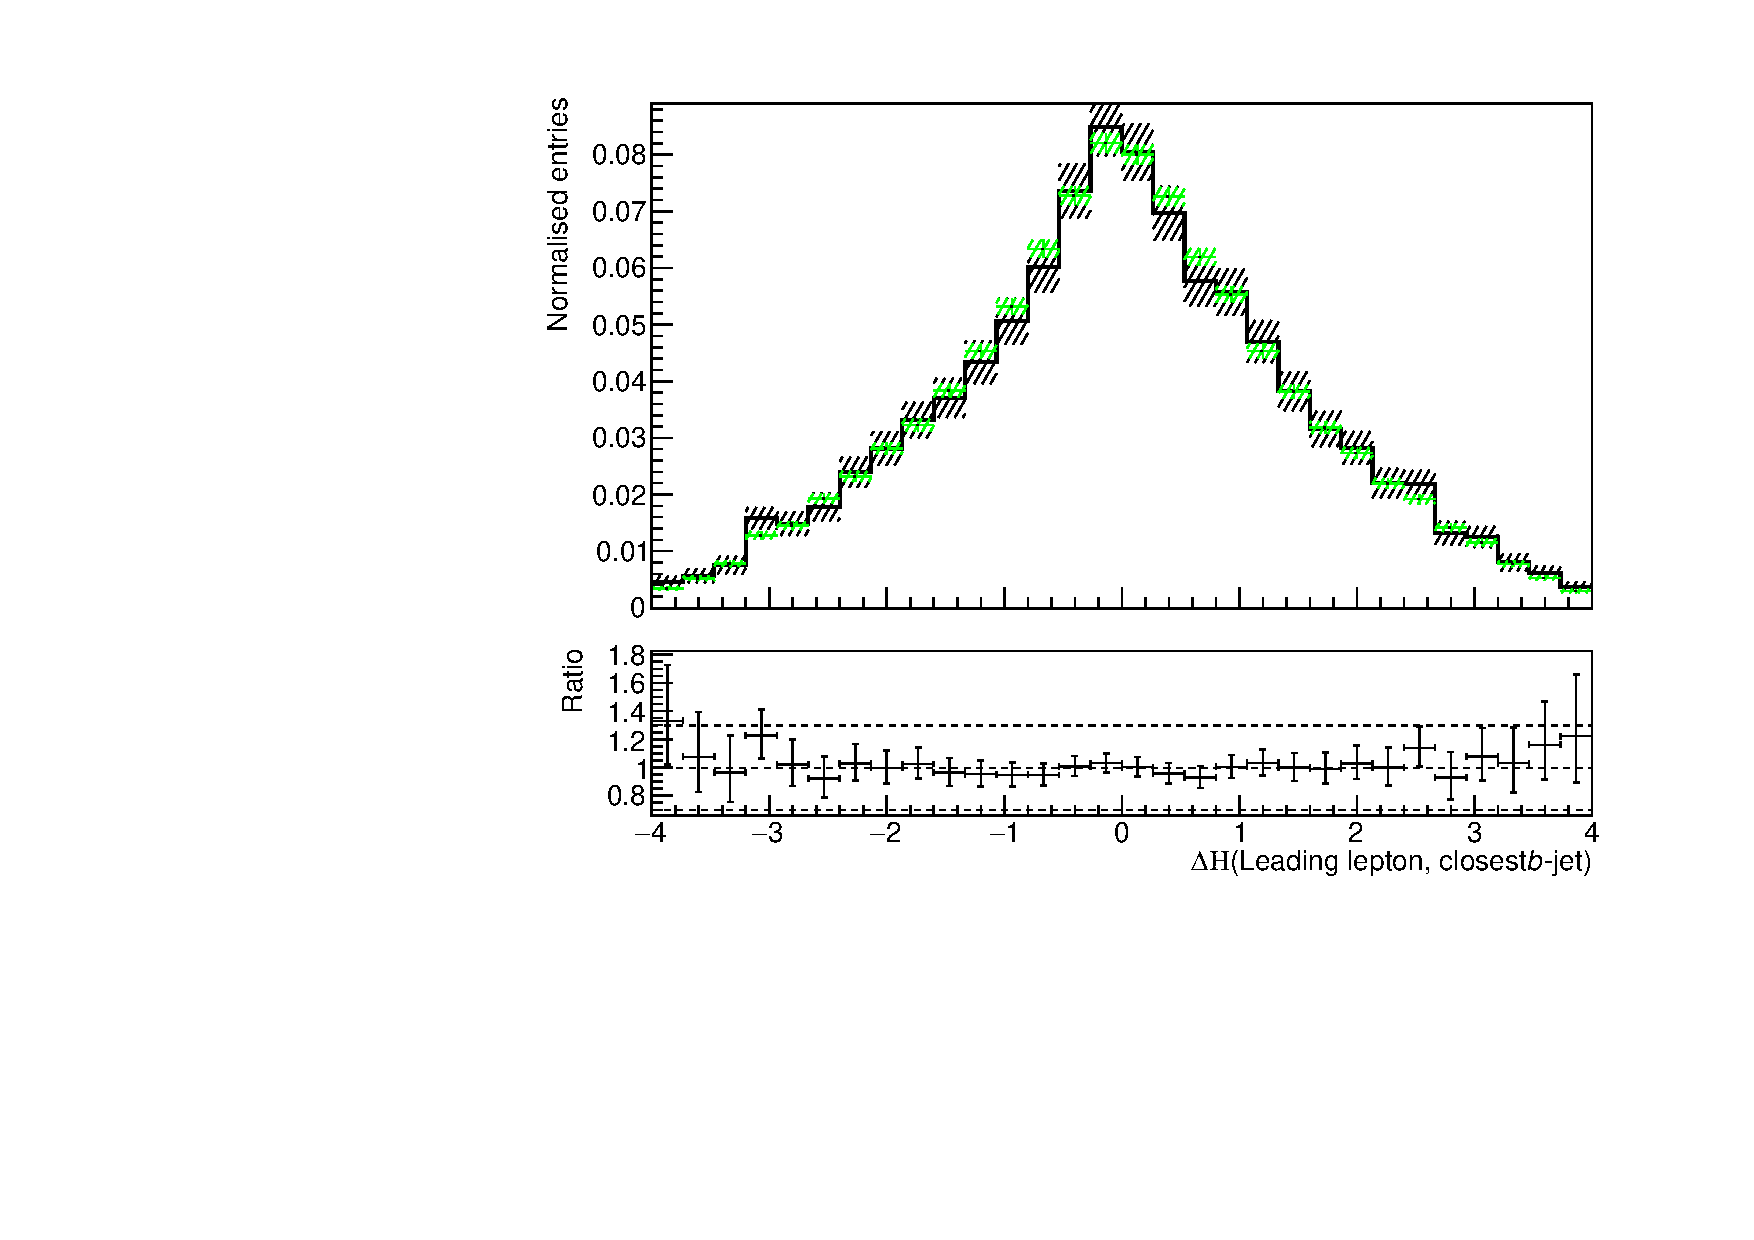
\includegraphics[width=.95\linewidth]{Chapter5_tHq/LeptAssociation/NegativeWeights/PosVsAll_SS_err_DeltaEtaLeadingLeptonClosestBjet}
  %\caption{}
\end{subfigure}%
\begin{subfigure}{.46\textwidth}
  \centering
  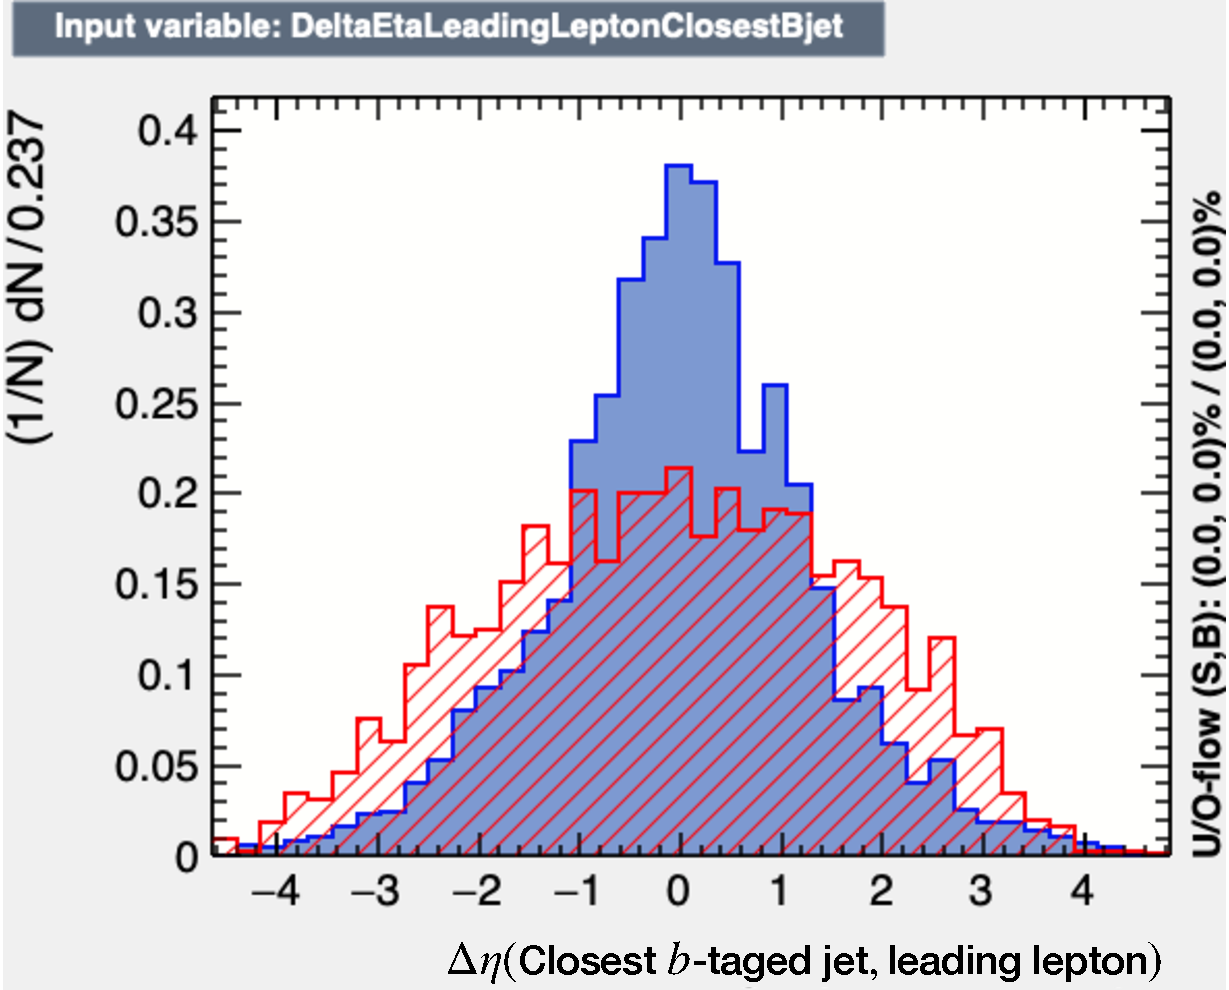
\includegraphics[width=.95\linewidth]{Chapter5_tHq/LeptAssociation/BDT_InputVariables/pdf_input_DeltaEtaLeadingLeptonClosestBjet}
  %\caption{}
\end{subfigure}
\caption{Normalised distributions for $\Delta \eta(\text{closest }b\text{-taged jet}, \text{leading lepton})$.}
\label{fig:Appendix:BDTVARS:LeptonAssignment:DeltaEtaLeadingLeptonClosestBjet}
\end{figure}



\FloatBarrier


%%%%%%%%%%%%%%%%%
% 		tHq OS			%
%%%%%%%%%%%%%%%%%
\section{BDT$(\tHq|_{\text{OS}})$}
\label{chap:Appendix:BDT_Variables:OS_tHq}
For all distributions presented here, the uncertainty bands include the statistical and 
systematic uncertainties and the lower panel presents the ratio between the collected 
data and the MC simulation. Additionally, the $\chi^2$ measures the agreement between 
real and simulated data events.

When training an ML model, it is important to use variables that provide good modelling, i.e., good data/MC agreement.
For most of the distributions presented in the rest of the appendix, while the data/MC agreement is far from being exact,  
it is compatible with the uncertainty. The variables are presented in their order of importance within the BDT (see
Figure~\ref{fig:ChaptH:EventSelection:BDT:Rankings:tHqOS})

%\pablo{In this section i want that the separation plots separate tHq and the rest of the precesses.}

%\begin{figure}[h]
%  \centering
%  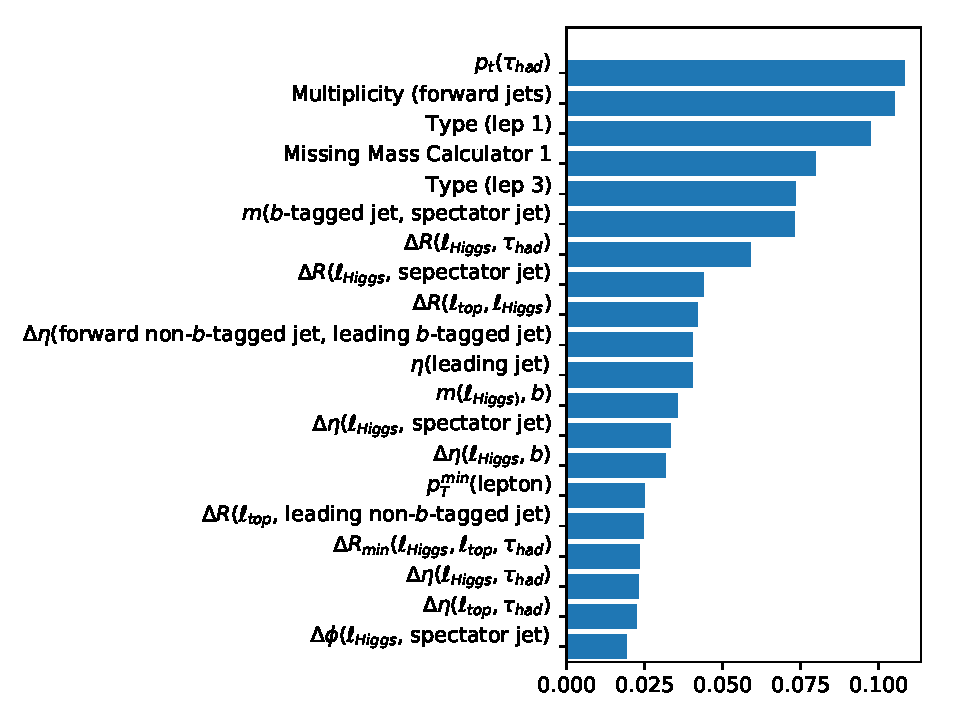
\includegraphics[width=.95\linewidth]{Chapter5_tHq/BDT_Results/Feature_importance_tHq_OS}
%\caption{Ranking of features for the BDT$(\tHq|_{\text{OS}})$}
%\label{fig:Appendix:BDTVARS:tHqOS:Feature_importance_tHq_OS}
%\end{figure}



\begin{figure}[h]
\centering
\begin{subfigure}{.47\textwidth}
  \centering
  \includegraphics[width=.95\linewidth]{Chapter5_tHq/BDT_Results/BDT_Variables_tHq_OS/Separation/a01_PR_had_tau_pt_2L1TAU_OS}
  \caption{}
\end{subfigure}%
\begin{subfigure}{.47\textwidth}
  \centering
  \includegraphics[width=.95\linewidth]{Chapter5_tHq/BDT_Results/BDT_Variables_tHq_OS/Separation/a02_PR_m_nfjets_2L1TAU_OS}
  \caption{}
\end{subfigure}
\caption{Separation plot for the two most discriminant variables of the BDT$(\tHq|_{\text{OS}})$.
The original distributions for these features are presented in Figure~\ref{fig:ChaptH:EventSelection:BDT:Top:tHqOS}.
In (a), the transverse momentum of the hadronically-decaying \Ptau-lepton is showed.
The reconstructed \tauhad is more boosted when it is produced from the Higgs-boson decay than in the main backgrounds. In (b), the number of forward jets present in the final state is swhon. A forward jet
is defined as a jet reconstructed within $2.5 < |\eta| < 4.5$.  The jets more forward than $|\eta| < 4.5$ are
not detected.
The forward jets are selected with the \textit{forward Jet Vertex Tagger}~\cite{ATLAS:2017ywy}.
The spectator-quark-initiated jet in the \tHq production is quite forward, so the multiplicity of forward jets peaks at one. 
In contrast, \ttbar and \Zjets do not have forward jets in hard-scattering process. }
\label{fig:Appendix:BDTVARS:tHqOS:BestTwo}
\end{figure}



\begin{comment}
\begin{figure}[h]
\centering
\begin{subfigure}{.45\textwidth}
  \centering
  \includegraphics[width=.95\linewidth]{Chapter5_tHq/BDT_Results/BDT_Variables_tHq_OS/a01_PR_had_tau_pt_2L1TAU_OS}
  %\caption{}
\end{subfigure}%
\begin{subfigure}{.55\textwidth}
  \centering
  \includegraphics[width=.95\linewidth]{Chapter5_tHq/BDT_Results/BDT_Variables_tHq_OS/Separation/a01_PR_had_tau_pt_2L1TAU_OS}
  %\caption{}
\end{subfigure}
\caption{Distribution and separation plot for the transverse momentum of the hadronically-decaying \Ptau-lepton.
The reconstructed \tauhad is more boosted when it is produced from the Higgs-boson decay than in the main backgrounds.
Note that there is a slight slope indicating an excess of MC prediction over the data as the \pT(\tauhad) increases.
This discrepancy is due to the scale factors accounting for the misidentification rates in \ttbar.}
\label{fig:Appendix:BDTVARS:tHqOS:a01_PR_had_tau_pt}
\end{figure}

\begin{figure}[h]
\centering
\begin{subfigure}{.45\textwidth}
  \centering
  \includegraphics[width=.95\linewidth]{Chapter5_tHq/BDT_Results/BDT_Variables_tHq_OS/a02_PR_m_nfjets_2L1TAU_OS}
  %\caption{}
\end{subfigure}%
\begin{subfigure}{.55\textwidth}
  \centering
  \includegraphics[width=.95\linewidth]{Chapter5_tHq/BDT_Results/BDT_Variables_tHq_OS/Separation/a02_PR_m_nfjets_2L1TAU_OS}
  %\caption{}
\end{subfigure}
\caption{Distribution and separation plot for the number of forward jets present in the final state. A forward jet
is defined as a jet reconstructed within $2.5 < |\eta| < 4.5$.  The jets more forward than $|\eta| < 4.5$ are
not detected.
The forward jets are selected with the \textit{forward Jet Vertex Tagger}~\cite{ATLAS:2017ywy}.
The spectator-quark-initiated jet in the \tHq production is quite forward, so the multiplicity of forward jets peaks at one. 
In contrast, \ttbar and \Zjets do not have forward jets in hard-scattering process. 
Note that there is a tendency to have an excess of data over the MC as the forward jet multiplicity increases.
This discrepancy is not present on the SR(\tHq) but only on the dedicated regions for \ttbar and \Zjets.}
\label{fig:Appendix:BDTVARS:tHqOS:a02_PR_m_nfjets}
\end{figure}
\end{comment}


\begin{figure}[h]
\centering
\begin{subfigure}{.45\textwidth}
  \centering
  \includegraphics[width=.95\linewidth]{Chapter5_tHq/BDT_Results/BDT_Variables_tHq_OS/a03_PR_type_lep1_2L1TAU_OS}
  %\caption{}
\end{subfigure}%
\begin{subfigure}{.55\textwidth}
  \centering
  \includegraphics[width=.95\linewidth]{Chapter5_tHq/BDT_Results/BDT_Variables_tHq_OS/Separation/a03_PR_type_lep1_2L1TAU_OS}
  %\caption{}
\end{subfigure}
\caption{Distribution and separation plot for the flavour of the leading lepton. The types are 
\Pelectron/\APelectron (1), \Pmuon/\APmuon (2), and \Ptauon/\APtauon(3). Note that, for the backgrounds,
the reconstructed \tauhad rarely is the leading lepton. In contrast, for the \tHq production, the 
flavour of the leading lepton is more distributed.
There is a disagreement between data and MC prediction for the events in which the \tauhad is the leading lepton (third bin), this
can be linked with the phenomena observed in Figure~\ref{fig:ChaptH:EventSelection:BDT:Top:tHqOS:pt}, in which the modelling
of the \pt(\tauhad) misbehave for large \pT. } 
\label{fig:Appendix:BDTVARS:tHqOS:a03_PR_type_lep1}
\end{figure}

\begin{figure}[h]
\centering
\begin{subfigure}{.45\textwidth}
  \centering
  \includegraphics[width=.95\linewidth]{Chapter5_tHq/BDT_Results/BDT_Variables_tHq_OS/a04_PR_MMC_out_1_2L1TAU_OS}
  %\caption{}
\end{subfigure}%
\begin{subfigure}{.55\textwidth}
  \centering
  \includegraphics[width=.95\linewidth]{Chapter5_tHq/BDT_Results/BDT_Variables_tHq_OS/Separation/a04_PR_MMC_out_1_2L1TAU_OS}
  %\caption{}
\end{subfigure}
\caption{Distribution and separation plot for the reconstructed mass of the Higgs boson 
using the MMC method~\cite{ELAGIN2011481}. It peaks around $125.25\pm0.17$~GeV, which corresponds to \mH~\cite{Workman:2022ynf}.  %~\cite{pdgHiggs}.
This variable allows to separate events with a real Higgs boson (e.g. \tWH, \tHq, \ttH) from the rest.}
\label{fig:Appendix:BDTVARS:tHqOS:a04_PR_MMC_out_1}
\end{figure}

\begin{figure}[h]
\centering
\begin{subfigure}{.45\textwidth}
  \centering
  \includegraphics[width=.95\linewidth]{Chapter5_tHq/BDT_Results/BDT_Variables_tHq_OS/a05_PR_type_lep3_2L1TAU_OS}
  %\caption{}
\end{subfigure}%
\begin{subfigure}{.55\textwidth}
  \centering
  \includegraphics[width=.95\linewidth]{Chapter5_tHq/BDT_Results/BDT_Variables_tHq_OS/Separation/a05_PR_type_lep3_2L1TAU_OS}
  %\caption{}
\end{subfigure}
\caption{Distribution and separation plot for the flavour type of the sub-sub-leading lepton. 
In Figure~\ref{fig:Appendix:BDTVARS:tHqOS:a03_PR_type_lep1} is observed that,
for the backgrounds,
the \tauhad does not  tend to be the leading lepton. In agreement, this Figure shows 
that the \tauhad typically is the lepton with lower \pT for the backgrounds.
However, this is not the case for the \tHq production.
Observe that Type($\ell_{1}$) and Type($\ell_{2}$) are the only features that use the \pT-based definition to refer to the light leptons.}
\label{fig:Appendix:BDTVARS:tHqOS:a05_PR_type_lep3}
\end{figure}

\begin{figure}[h]
\centering
\begin{subfigure}{.45\textwidth}
  \centering
  \includegraphics[width=.95\linewidth]{Chapter5_tHq/BDT_Results/BDT_Variables_tHq_OS/a06_PR_m_inv_bjet_spectjet_2L1TAU_OS}
  %\caption{}
\end{subfigure}%
\begin{subfigure}{.55\textwidth}
  \centering
  \includegraphics[width=.95\linewidth]{Chapter5_tHq/BDT_Results/BDT_Variables_tHq_OS/Separation/a06_PR_m_inv_bjet_spectjet_2L1TAU_OS}
  %\caption{}
\end{subfigure}
\caption{Distribution and separation plot for the invariant mass of the leading \btagged jet and the spectator jet.
The spectator jet is the one produced by the quark that is scattered in the Feynman diagrams of 
Figures~\ref{fig:Chap1:tHq:Feynman_LO_top} and \ref{fig:Chap1:tHq:Feynman_LO_W}.}
\label{fig:Appendix:BDTVARS:tHqOS:a06_PR_m_inv_bjet_spectjet}
\end{figure}

\begin{figure}[h]
\centering
\begin{subfigure}{.45\textwidth}
  \centering
  \includegraphics[width=.95\linewidth]{Chapter5_tHq/BDT_Results/BDT_Variables_tHq_OS/a07_PR_DeltaR_lepHiggs_tau_2L1TAU_OS}
  %\caption{}
\end{subfigure}%
\begin{subfigure}{.55\textwidth}
  \centering
  \includegraphics[width=.95\linewidth]{Chapter5_tHq/BDT_Results/BDT_Variables_tHq_OS/Separation/a07_PR_DeltaR_lepHiggs_tau_2L1TAU_OS}
  %\caption{}
\end{subfigure}
\caption{Distribution and separation plot for the $\Delta R$ distance between the $\ell_{\text{Higgs}}$ and the \tauhad. 
Since in the \tHq process the $\ell_{\text{Higgs}}$ and the \tauhad are direct-decay products of the Higgs boson (83.71\% of times as calculated in Table~\ref{tab:ChaptH:TruthSummary})
they tend to be geometrically close.}
\label{fig:Appendix:BDTVARS:tHqOS:a07_PR_DeltaR_lepHiggs_tau}
\end{figure}

\begin{figure}[h]
\centering
\begin{subfigure}{.45\textwidth}
  \centering
  \includegraphics[width=.95\linewidth]{Chapter5_tHq/BDT_Results/BDT_Variables_tHq_OS/a08_PR_deltaR_lepHiggs_spectatorJet_2L1TAU_OS}
  %\caption{}
\end{subfigure}%
\begin{subfigure}{.55\textwidth}
  \centering
  \includegraphics[width=.95\linewidth]{Chapter5_tHq/BDT_Results/BDT_Variables_tHq_OS/Separation/a08_PR_deltaR_lepHiggs_spectatorJet_2L1TAU_OS}
  %\caption{}
\end{subfigure}
\caption{Distribution and separation plot for the $\Delta R$ distance between the $\ell_{\text{Higgs}}$ and
spectator jet. }
\label{fig:Appendix:BDTVARS:tHqOS:a08_PR_deltaR_lepHiggs_spectatorJet}
\end{figure}

\begin{figure}[h]
\centering
\begin{subfigure}{.45\textwidth}
  \centering
  \includegraphics[width=.95\linewidth]{Chapter5_tHq/BDT_Results/BDT_Variables_tHq_OS/a09_PR_DeltaR_lepTop_lepHiggs_2L1TAU_OS}
  %\caption{}
\end{subfigure}%
\begin{subfigure}{.55\textwidth}
  \centering
  \includegraphics[width=.95\linewidth]{Chapter5_tHq/BDT_Results/BDT_Variables_tHq_OS/Separation/a09_PR_DeltaR_lepTop_lepHiggs_2L1TAU_OS}
  %\caption{}
\end{subfigure}
\caption{Distribution and separation plot for the $\Delta R$ distance between the two charged light-flavoured leptons.}
%The events of the signal are more blablabla}
\label{fig:Appendix:BDTVARS:tHqOS:a09_PR_DeltaR_lepTop_lepHiggs}
\end{figure}

\begin{figure}[h]
\centering
\begin{subfigure}{.45\textwidth}
  \centering
  \includegraphics[width=.95\linewidth]{Chapter5_tHq/BDT_Results/BDT_Variables_tHq_OS/a10_PR_DeltaEtaForwardLjetLeadingBjet_2L1TAU_OS}
  %\caption{}
\end{subfigure}%
\begin{subfigure}{.55\textwidth}
  \centering
  \includegraphics[width=.95\linewidth]{Chapter5_tHq/BDT_Results/BDT_Variables_tHq_OS/Separation/a10_PR_DeltaEtaForwardLjetLeadingBjet_2L1TAU_OS}
  %\caption{}
\end{subfigure}
\caption{Distribution and separation plot for the $\Delta \eta$ distance between the forward non-\btagged jet
and the leading \btagged jet. The non-\btagged jets are also referred as light jets.}
\label{fig:Appendix:BDTVARS:tHqOS:a10_PR_DeltaEtaForwardLjetLeadingBjet}
\end{figure}

\begin{figure}[h]
\centering
\begin{subfigure}{.45\textwidth}
  \centering
  \includegraphics[width=.95\linewidth]{Chapter5_tHq/BDT_Results/BDT_Variables_tHq_OS/a11_PR_eta_jet1_2L1TAU_OS}
  %\caption{}
\end{subfigure}%
\begin{subfigure}{.55\textwidth}
  \centering
  \includegraphics[width=.95\linewidth]{Chapter5_tHq/BDT_Results/BDT_Variables_tHq_OS/Separation/a11_PR_eta_jet1_2L1TAU_OS}
  %\caption{}
\end{subfigure}
\caption{Distribution and separation plot for the $\eta$ of the leading jet, which typically is more forward for
the \tHq process than for the backgrounds.}
\label{fig:Appendix:BDTVARS:tHqOS:a11_PR_eta_jet1}
\end{figure}

\begin{figure}[h]
\centering
\begin{subfigure}{.45\textwidth}
  \centering
  \includegraphics[width=.95\linewidth]{Chapter5_tHq/BDT_Results/BDT_Variables_tHq_OS/a12_PR_m_lepHiggs_b_2L1TAU_OS}
  %\caption{}
\end{subfigure}%
\begin{subfigure}{.55\textwidth}
  \centering
  \includegraphics[width=.95\linewidth]{Chapter5_tHq/BDT_Results/BDT_Variables_tHq_OS/Separation/a12_PR_m_lepHiggs_b_2L1TAU_OS}
  %\caption{}
\end{subfigure}
\caption{Distribution and separation plot for the invariant mass of the $\ell_{\text{Higgs}}$ and the leading \btagged jet. This one is the 
only variable shared between the BDT$(\tHq|_{\text{OS}})$ and the BDT$(\ttbar|_{\text{OS}})$.}
\label{fig:Appendix:BDTVARS:tHqOS:a12_PR_m_lepHiggs_b}
\end{figure}

\begin{figure}[h]
\centering
\begin{subfigure}{.45\textwidth}
  \centering
  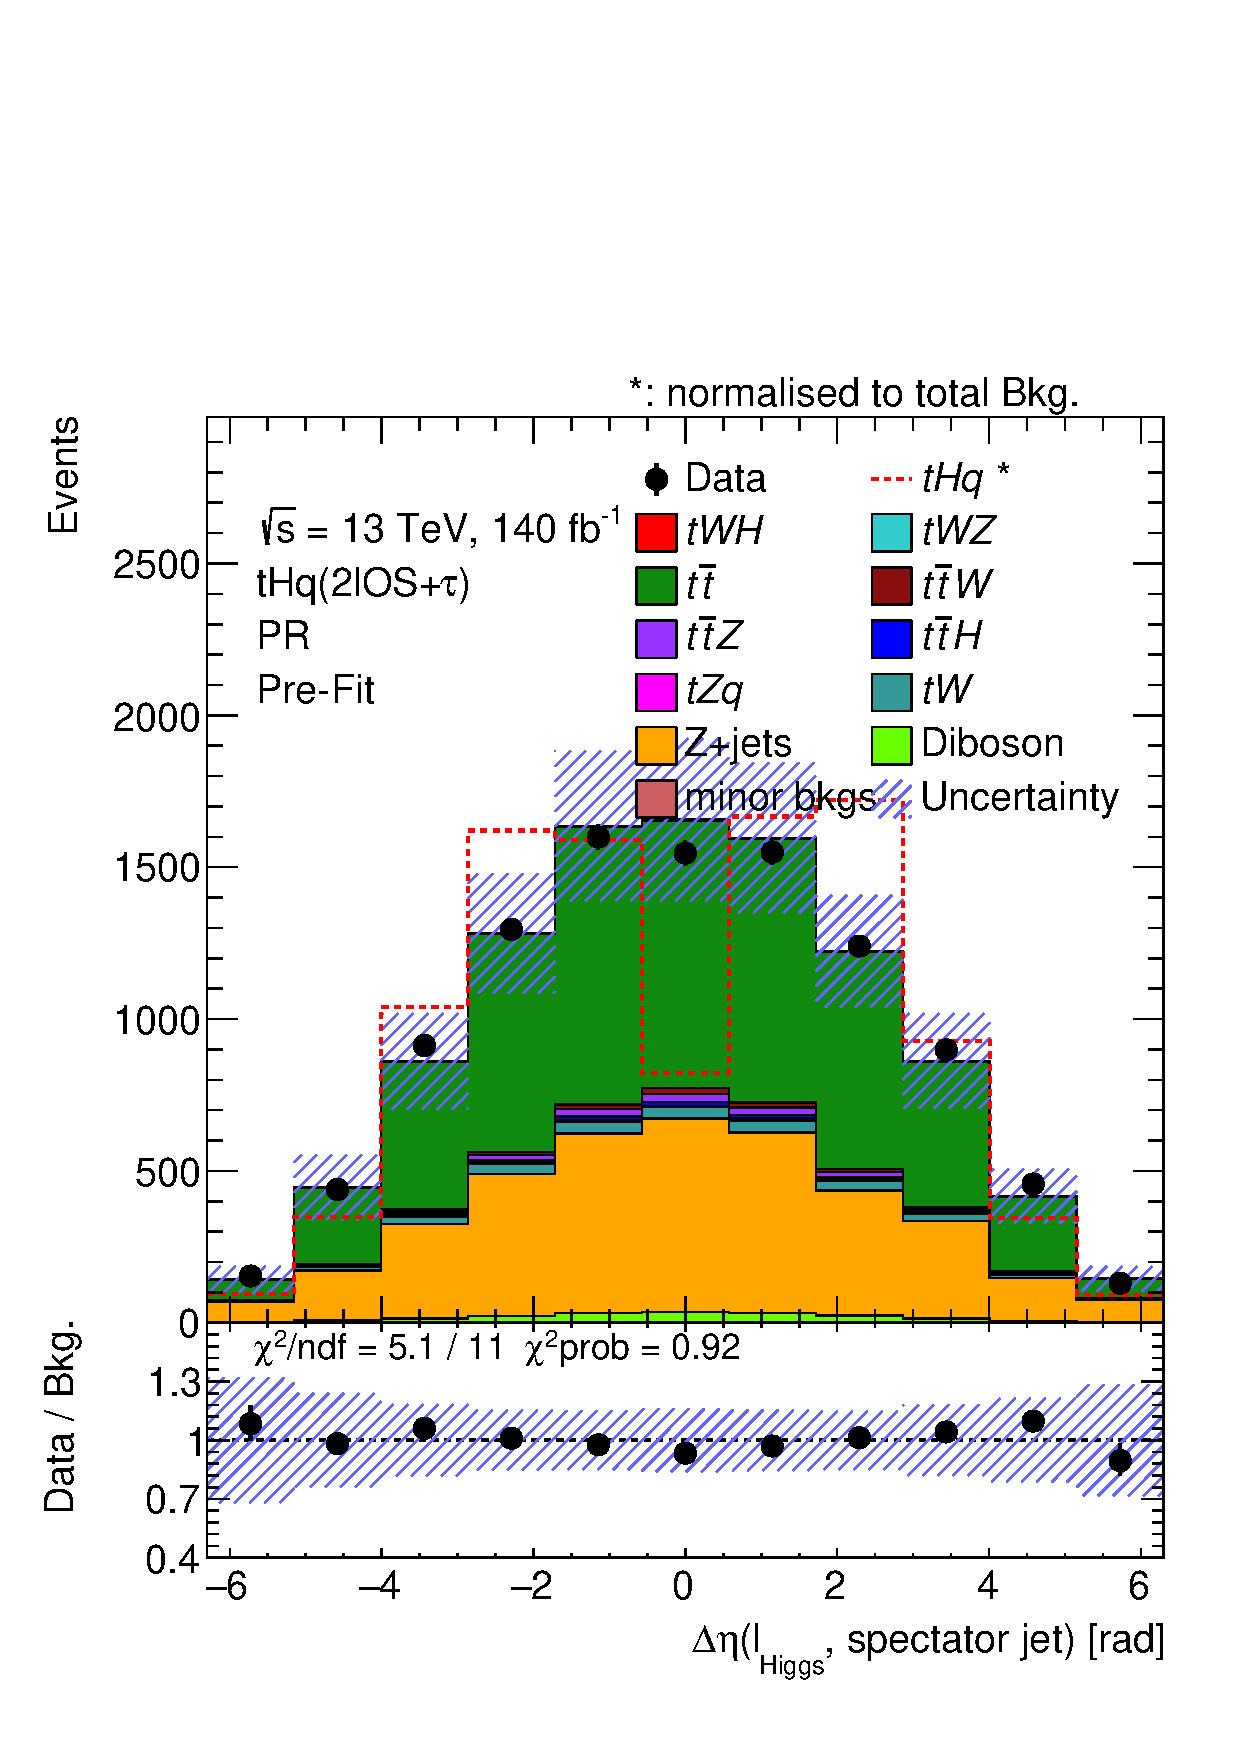
\includegraphics[width=.95\linewidth]{Chapter5_tHq/BDT_Results/BDT_Variables_tHq_OS/a13_PR_deltaEta_lepHiggs_spectatorJet_2L1TAU_OS}
  %\caption{}
\end{subfigure}%
\begin{subfigure}{.55\textwidth}
  \centering
  \includegraphics[width=.95\linewidth]{Chapter5_tHq/BDT_Results/BDT_Variables_tHq_OS/Separation/a13_PR_deltaEta_lepHiggs_spectatorJet_2L1TAU_OS}
  %\caption{}
\end{subfigure}
\caption{Distribution and separation plot for the $\Delta \eta$ distance between the $\ell_{\text{Higgs}}$ and
the jet initiated by the spectator quark.}
\label{fig:Appendix:BDTVARS:tHqOS:a13_PR_deltaEta_lepHiggs_spectatorJet}
\end{figure}

\begin{figure}[h]
\centering
\begin{subfigure}{.45\textwidth}
  \centering
  \includegraphics[width=.95\linewidth]{Chapter5_tHq/BDT_Results/BDT_Variables_tHq_OS/a14_PR_DeltaEta_lepHiggs_b_2L1TAU_OS}
  %\caption{}
\end{subfigure}%
\begin{subfigure}{.55\textwidth}
  \centering
  \includegraphics[width=.95\linewidth]{Chapter5_tHq/BDT_Results/BDT_Variables_tHq_OS/Separation/a14_PR_DeltaEta_lepHiggs_b_2L1TAU_OS}
  %\caption{}
\end{subfigure}
\caption{Distribution and separation plot for the $\Delta \eta$ distance between the $\ell_{\text{Higgs}}$ and 
the leading \btagged jet.}
\label{fig:Appendix:BDTVARS:tHqOS:a14_PR_DeltaEta_lepHiggs_b}
\end{figure}

\begin{figure}[h]
\centering
\begin{subfigure}{.45\textwidth}
  \centering
  \includegraphics[width=.95\linewidth]{Chapter5_tHq/BDT_Results/BDT_Variables_tHq_OS/a15_PR_PtLeptonMin_2L1TAU_OS}
  %\caption{}
\end{subfigure}%
\begin{subfigure}{.55\textwidth}
  \centering
  \includegraphics[width=.95\linewidth]{Chapter5_tHq/BDT_Results/BDT_Variables_tHq_OS/Separation/a15_PR_PtLeptonMin_2L1TAU_OS}
  %\caption{}
\end{subfigure}
\caption{Distribution and separation plot of the \pT of the softest lepton (including \Ptau-flavoured leptons).}
\label{fig:Appendix:BDTVARS:tHqOS:a15_PR_PtLeptonMin}
\end{figure}

\begin{figure}[h]
\centering
\begin{subfigure}{.45\textwidth}
  \centering
  \includegraphics[width=.95\linewidth]{Chapter5_tHq/BDT_Results/BDT_Variables_tHq_OS/a16_PR_deltaR_lepTop_leadingLjet_2L1TAU_OS}
  %\caption{}
\end{subfigure}%
\begin{subfigure}{.55\textwidth}
  \centering
  \includegraphics[width=.95\linewidth]{Chapter5_tHq/BDT_Results/BDT_Variables_tHq_OS/Separation/a16_PR_deltaR_lepTop_leadingLjet_2L1TAU_OS}
  %\caption{}
\end{subfigure}
\caption{Distribution and separation plot for the $\Delta R$ distance between the $\ell_{\text{top}}$ and
the leading non-\btagged jet.}
\label{fig:Appendix:BDTVARS:tHqOS:a16_PR_deltaR_lepTop_leadingLjet}
\end{figure}

\begin{figure}[h]
\centering
\begin{subfigure}{.45\textwidth}
  \centering
  \includegraphics[width=.95\linewidth]{Chapter5_tHq/BDT_Results/BDT_Variables_tHq_OS/a17_PR_DeltaRMin_2L1TAU_OS}
  %\caption{}
\end{subfigure}%
\begin{subfigure}{.55\textwidth}
  \centering
  \includegraphics[width=.95\linewidth]{Chapter5_tHq/BDT_Results/BDT_Variables_tHq_OS/Separation/a17_PR_DeltaRMin_2L1TAU_OS}
  %\caption{}
\end{subfigure}
\caption{Distribution and separation plot for the minimum $\Delta R$ distance between any two charged leptons form the 
the three that are present in the final state.}
\label{fig:Appendix:BDTVARS:tHqOS:a17_PR_DeltaRMin}
\end{figure}

\begin{figure}[h]
\centering
\begin{subfigure}{.45\textwidth}
  \centering
  \includegraphics[width=.95\linewidth]{Chapter5_tHq/BDT_Results/BDT_Variables_tHq_OS/a18_PR_DeltaEta_lepHiggs_tau_2L1TAU_OS}
  %\caption{}
\end{subfigure}%
\begin{subfigure}{.55\textwidth}
  \centering
  \includegraphics[width=.95\linewidth]{Chapter5_tHq/BDT_Results/BDT_Variables_tHq_OS/Separation/a18_PR_DeltaEta_lepHiggs_tau_2L1TAU_OS}
  %\caption{}
\end{subfigure}
\caption{Distribution and separation plot for the $\Delta \eta$ distance between the $\ell_{\text{Higgs}}$ and
the \tauhad.}
\label{fig:Appendix:BDTVARS:tHqOS:a18_PR_DeltaEta_lepHiggs_tau}
\end{figure}

\begin{figure}[h]
\centering
\begin{subfigure}{.45\textwidth}
  \centering
  \includegraphics[width=.95\linewidth]{Chapter5_tHq/BDT_Results/BDT_Variables_tHq_OS/a19_PR_DeltaEta_lepTop_tau_2L1TAU_OS}
  %\caption{}
\end{subfigure}%
\begin{subfigure}{.55\textwidth}
  \centering
  \includegraphics[width=.95\linewidth]{Chapter5_tHq/BDT_Results/BDT_Variables_tHq_OS/Separation/a19_PR_DeltaEta_lepTop_tau_2L1TAU_OS}
  %\caption{}
\end{subfigure}
\caption{Distribution and separation plot for the $\Delta R$ distance between the $\ell_{\text{top}}$ and \tauhad.}
\label{fig:Appendix:BDTVARS:tHqOS:a19_PR_DeltaEta_lepTop_tau}
\end{figure}

\begin{figure}[h]
\centering
\begin{subfigure}{.45\textwidth}
  \centering
  \includegraphics[width=.95\linewidth]{Chapter5_tHq/BDT_Results/BDT_Variables_tHq_OS/a20_PR_deltaPhi_lepHiggs_spectatorJet_2L1TAU_OS}
  %\caption{}
\end{subfigure}%
\begin{subfigure}{.55\textwidth}
  \centering
  \includegraphics[width=.95\linewidth]{Chapter5_tHq/BDT_Results/BDT_Variables_tHq_OS/Separation/a20_PR_deltaPhi_lepHiggs_spectatorJet_2L1TAU_OS}
  %\caption{}
\end{subfigure}
\caption{Distribution and separation plot for the $\Delta \phi$ distance between the $\ell_{\text{Higgs}}$ and
the spectator jet.}
\label{fig:Appendix:BDTVARS:tHqOS:a20_PR_deltaPhi_lepHiggs_spectatorJet}
\end{figure}

\FloatBarrier


%%%%%%%%%%%%%%%%%
% 		ttbar OS			%
%%%%%%%%%%%%%%%%%
\section{BDT$(\ttbar|_{\text{OS}})$}
\label{chap:Appendix:BDT_Variables:OS_ttbar}
This model aims to separate the \ttbar and \Zjets processes to 
define dedicated regions. Therefore, the variables presented are those that
can discriminate between these two backgrounds.


As well as for the distributions above, the uncertainties included here correspond
to both the statistical and systematic ones, and the lower panel presents the ratio 
between the collected data and the MC simulation. 
The variables are presented in their order of importance for the BDT$(\ttbar|_{\text{OS}})$, as
Figure~\ref{fig:ChaptH:EventSelection:BDT:Rankings:ttbarOS} presents. 
%\pablo{In this section i want that the separation plots separate ttbar, Zjets and tHq}

%\begin{figure}[h]
%  \centering
%  \includegraphics[width=.75\linewidth]{Chapter5_tHq/BDT_Results/Feature_importance_ttbar_OS__ReplicateOldModel}
%\caption{Ranking of features for the BDT$(\ttbar |_{\text{OS}})$. The main purpose of this BDT is to discriminate
%between the two dominant backgrounds in the \dilepOStau channel \ttbar and \Zjets.}
%\label{fig:Appendix:BDTVARS:tHqOS:Feature_importance_ttbar_OS}
%\end{figure}


\begin{figure}[h]
\centering
\begin{subfigure}{.47\textwidth}
  \centering
  \includegraphics[width=.95\linewidth]{Chapter5_tHq/BDT_Results/BDT_Variables_ttbar_OS/Separation/a01_PR_lep_top_higgs_mass_2L1TAU_OS}
  %\caption{}
\end{subfigure}%
\begin{subfigure}{.47\textwidth}
  \centering
  \includegraphics[width=.95\linewidth]{Chapter5_tHq/BDT_Results/BDT_Variables_ttbar_OS/Separation/a02_PR_MET_2L1TAU_OS}
  %\caption{}
\end{subfigure}
\caption{Separation plot for the two input features with highest discriminant power in the BDT$(\ttbar|_{\text{OS}})$.
The distributions for these two variables showing all processes are presented in Figure~\ref{fig:ChaptH:EventSelection:BDT:Top:ttbarOS}.
In (a), the invariant mass of the two charged light-flavoured leptons is presented.
The peak around $m(\ell_{\text{Higgs}}, \ell_{\text{top}})=90$~GeV corresponds to the events in which a 
\PZ boson is produced. The mass of the \PZ is $m_{\PZ} = (91.1876 \pm 0.0021)$~GeV~\cite{Workman:2022ynf} and %~\cite{pdgZ_mass}
when the mass of the light leptons produced in the \PZ-boson decay is reconstructed, values close
to $m_{\PZ}$ are obtained. Therefore, this variable allows us to identify \Zjets processes.
The \MET separation plot is shown in (b). Note that while this variable provides 
good discrimination power against \Zjets, it was not able to separate \ttbar and \tHq.
For this reason, in the studies in which \MET is introduced  for the training of the BDT$(\tHq|_{\text{OS}})$,
the model becomes specialised in discriminating \tHq and \Zjets but the separation between 
\tHq and \ttbar gets worse.}
\label{fig:Appendix:BDTVARS:ttbarOS:BestTwo}
\end{figure}


\begin{comment}
\begin{figure}[h]
\centering
\begin{subfigure}{.45\textwidth}
  \centering
  \includegraphics[width=.95\linewidth]{Chapter5_tHq/BDT_Results/BDT_Variables_ttbar_OS/a01_PR_lep_top_higgs_mass_2L1TAU_OS}
  %\caption{}
\end{subfigure}%
\begin{subfigure}{.55\textwidth}
  \centering
  \includegraphics[width=.95\linewidth]{Chapter5_tHq/BDT_Results/BDT_Variables_ttbar_OS/Separation/a01_PR_lep_top_higgs_mass_2L1TAU_OS}
  %\caption{}
\end{subfigure}
\caption{Distribution and separation plot for the invariant mass of the two charged light-flavoured leptons.
The peak around $m(\ell_{\text{Higgs}}, \ell_{\text{top}})=90$~GeV corresponds to the events in which a 
\PZ boson is produced. The mass of the \PZ is $m_{\PZ} = (91.1876 \pm 0.0021)$~GeV~\cite{Workman:2022ynf} and %~\cite{pdgZ_mass}
when the mass of the light leptons produced in the \PZ-boson decay is reconstructed, values close
to $m_{\PZ}$ are obtained. Therefore, this variable allows us to identify \Zjets processes.}
\label{fig:Appendix:BDTVARS:ttbarOS:a01_PR_lep_top_higgs_mass}
\end{figure}

\begin{figure}[h]
\centering
\begin{subfigure}{.45\textwidth}
  \centering
  \includegraphics[width=.95\linewidth]{Chapter5_tHq/BDT_Results/BDT_Variables_ttbar_OS/a02_PR_MET_2L1TAU_OS}
  %\caption{}
\end{subfigure}%
\begin{subfigure}{.55\textwidth}
  \centering
  \includegraphics[width=.95\linewidth]{Chapter5_tHq/BDT_Results/BDT_Variables_ttbar_OS/Separation/a02_PR_MET_2L1TAU_OS}
  %\caption{}
\end{subfigure}
\caption{Distribution and separation plot for the \MET. Note that while this variable provides 
good discrimination power against \Zjets, it was not able to separate \ttbar and \tHq.
For this reason, in the studies in which \MET is introduced  for the training of the BDT$(\tHq|_{\text{OS}})$,
the model becomes specialised in discriminating \tHq and \Zjets but the separation between 
\tHq and \ttbar gets worse.} 
\label{fig:Appendix:BDTVARS:ttbarOS:a02_PR_MET}
\end{figure}
\end{comment}

\begin{figure}[h]
\centering
\begin{subfigure}{.45\textwidth}
  \centering
  \includegraphics[width=.95\linewidth]{Chapter5_tHq/BDT_Results/BDT_Variables_ttbar_OS/a03_PR_pt_b_2L1TAU_OS}
  %\caption{}
\end{subfigure}%
\begin{subfigure}{.55\textwidth}
  \centering
  \includegraphics[width=.95\linewidth]{Chapter5_tHq/BDT_Results/BDT_Variables_ttbar_OS/Separation/a03_PR_pt_b_2L1TAU_OS}
  %\caption{}
\end{subfigure}
\caption{Distribution and separation plot for the \pT of the leading \btagged jet.}
\label{fig:Appendix:BDTVARS:ttbarOS:a03_PR_pt_b}
\end{figure}

\begin{figure}[h]
\centering
\begin{subfigure}{.45\textwidth}
  \centering
  \includegraphics[width=.95\linewidth]{Chapter5_tHq/BDT_Results/BDT_Variables_ttbar_OS/a04_PR_m_lepHiggs_b_2L1TAU_OS}
  %\caption{}
\end{subfigure}%
\begin{subfigure}{.55\textwidth}
  \centering
  \includegraphics[width=.95\linewidth]{Chapter5_tHq/BDT_Results/BDT_Variables_ttbar_OS/Separation/a04_PR_m_lepHiggs_b_2L1TAU_OS}
  %\caption{}
\end{subfigure}
\caption{Distribution and separation plot for the invariant mass of the $\ell_{\text{Higgs}}$ and the leading \btagged jet.
This variable is also present in the training of the BDT$(\tHq|_{\text{OS}})$.}
\label{fig:Appendix:BDTVARS:ttbarOS:a04_PR_m_lepHiggs_b}
\end{figure}

\begin{figure}[h]
\centering
\begin{subfigure}{.45\textwidth}
  \centering
  \includegraphics[width=.95\linewidth]{Chapter5_tHq/BDT_Results/BDT_Variables_ttbar_OS/a05_PR_TvisMass_2L1TAU_OS}
  %\caption{}
\end{subfigure}%
\begin{subfigure}{.55\textwidth}
  \centering
  \includegraphics[width=.95\linewidth]{Chapter5_tHq/BDT_Results/BDT_Variables_ttbar_OS/Separation/a05_PR_TvisMass_2L1TAU_OS}
  %\caption{}
\end{subfigure}
\caption{Distribution and separation plot for the visible mass of the reconstructed top quark. 
The visible mass refers to the sum of the mass of all particles that are not neutrinos that decayed form the top quark.}
\label{fig:Appendix:BDTVARS:ttbarOS:a05_PR_TvisMass}
\end{figure}

\begin{figure}[h]
\centering
\begin{subfigure}{.45\textwidth}
  \centering
  \includegraphics[width=.95\linewidth]{Chapter5_tHq/BDT_Results/BDT_Variables_ttbar_OS/a06_PR_m_btagbin_jet1_2L1TAU_OS}
  %\caption{}
\end{subfigure}%
\begin{subfigure}{.55\textwidth}
  \centering
  \includegraphics[width=.95\linewidth]{Chapter5_tHq/BDT_Results/BDT_Variables_ttbar_OS/Separation/a06_PR_m_btagbin_jet1_2L1TAU_OS}
  %\caption{}
\end{subfigure}
\caption{Distribution and separation plot for binned DL1r score (calibrated) of the leading \btagged jet~\cite{ATLAS:2017gpy}. 
In Equation~\ref{eq:Chap3:DL1r_discriminant} the formulation of the DL1r score is presented.}
\label{fig:Appendix:BDTVARS:ttbarOS:a06_PR_m_btagbin_jet1}
\end{figure}

\begin{figure}[h]
\centering
\begin{subfigure}{.45\textwidth}
  \centering
  \includegraphics[width=.95\linewidth]{Chapter5_tHq/BDT_Results/BDT_Variables_ttbar_OS/a07_PR_pt_jet3_2L1TAU_OS}
  %\caption{}
\end{subfigure}%
\begin{subfigure}{.55\textwidth}
  \centering
  \includegraphics[width=.95\linewidth]{Chapter5_tHq/BDT_Results/BDT_Variables_ttbar_OS/Separation/a07_PR_pt_jet3_2L1TAU_OS}
  %\caption{}
\end{subfigure}
\caption{Distribution and separation plot for the \pT of the softest lepton.}
\label{fig:Appendix:BDTVARS:ttbarOS:a07_PR_pt_jet3}
\end{figure}

\begin{figure}[h]
\centering
\begin{subfigure}{.45\textwidth}
  \centering
  \includegraphics[width=.95\linewidth]{Chapter5_tHq/BDT_Results/BDT_Variables_ttbar_OS/a08_PR_m_btagbin_jet2_2L1TAU_OS}
  %\caption{}
\end{subfigure}%
\begin{subfigure}{.55\textwidth}
  \centering
  \includegraphics[width=.95\linewidth]{Chapter5_tHq/BDT_Results/BDT_Variables_ttbar_OS/Separation/a08_PR_m_btagbin_jet2_2L1TAU_OS}
  %\caption{}
\end{subfigure}
\caption{Distribution and separation plot for binned DL1r score (calibrated) of the sub-leading \btagged jet.}
\label{fig:Appendix:BDTVARS:ttbarOS:a08_PR_m_btagbin_jet2}
\end{figure}

\begin{figure}[h]
\centering
\begin{subfigure}{.45\textwidth}
  \centering
  \includegraphics[width=.95\linewidth]{Chapter5_tHq/BDT_Results/BDT_Variables_ttbar_OS/a10_PR_DeltaEtaForwardLjetSubLeadingBjet_2L1TAU_OS}
  %\caption{}
\end{subfigure}%
\begin{subfigure}{.55\textwidth}
  \centering
  \includegraphics[width=.95\linewidth]{Chapter5_tHq/BDT_Results/BDT_Variables_ttbar_OS/Separation/a10_PR_DeltaEtaForwardLjetSubLeadingBjet_2L1TAU_OS}
  %\caption{}
\end{subfigure}
\caption{Distribution and separation plot for the $\Delta \eta$ distance between the leading light jet and the subleading \btagged jet.}
\label{fig:Appendix:BDTVARS:ttbarOS:a10_PR_DeltaEtaForwardLjetSubLeadingBjet}
\end{figure}

\begin{figure}[h]
\centering
\begin{subfigure}{.45\textwidth}
  \centering
  \includegraphics[width=.95\linewidth]{Chapter5_tHq/BDT_Results/BDT_Variables_ttbar_OS/a10_PR_DeltaEta_lepTop_lepHiggs_2L1TAU_OS}
  %\caption{}
\end{subfigure}%
\begin{subfigure}{.55\textwidth}
  \centering
  \includegraphics[width=.95\linewidth]{Chapter5_tHq/BDT_Results/BDT_Variables_ttbar_OS/Separation/a10_PR_DeltaEta_lepTop_lepHiggs_2L1TAU_OS}
  %\caption{}
\end{subfigure}
\caption{Distribution and separation plot for the $\Delta \eta$ distance between the two light-flavoured-charged leptons. This
variable is also used in the BDT$(\tHq|_{\text{SS}})$.}
\label{fig:Appendix:BDTVARS:ttbarOS:a10_PR_DeltaEta_lepTop_lepHiggs}
\end{figure}

\begin{figure}[h]
\centering
\begin{subfigure}{.45\textwidth}
  \centering
  \includegraphics[width=.95\linewidth]{Chapter5_tHq/BDT_Results/BDT_Variables_ttbar_OS/a11_PR_DeltaEtaLeadingLeptonClosestBjet_2L1TAU_OS}
  %\caption{}
\end{subfigure}%
\begin{subfigure}{.55\textwidth}
  \centering
  \includegraphics[width=.95\linewidth]{Chapter5_tHq/BDT_Results/BDT_Variables_ttbar_OS/Separation/a11_PR_DeltaEtaLeadingLeptonClosestBjet_2L1TAU_OS}
  %\caption{}
\end{subfigure}
\caption{Distribution and separation plot for the $\Delta \eta$ distance between the leading lepton and the closest \btagged jet. Note
that this variable was also used in the training of the BDT$^{\text{Lepton Assignment}}$
(see Figure~\ref{fig:Appendix:BDTVARS:LeptonAssignment:DeltaEtaLeadingLeptonClosestBjet}).}
\label{fig:Appendix:BDTVARS:ttbarOS:a11_PR_DeltaEtaLeadingLeptonClosestBjet}
\end{figure}


\FloatBarrier

%%%%%%%%%%%%%%%%%
% 		tHq SS			%
%%%%%%%%%%%%%%%%%
\section{BDT$(\tHq|_{\text{SS}})$}
\label{chap:Appendix:BDT_Variables:SS_tHq}
The uncertainty bands depicted here encompass both statistical and systematic uncertainties. 
The lower panel illustrates the ratio between the actual data and the MC-simulated samples.
The variables are presented in their order of importance within the BDT$(\tHq|_{\text{SS}})$.
This ranking is presented in Figure~\ref{fig:ChaptH:EventSelection:BDT:Rankings:tHqSS})



%\begin{figure}[h]
%  \centering
%  \includegraphics[width=.75\linewidth]{Chapter5_tHq/BDT_Results/Feature_importance_tHq_SS_TestPaPonerEnTesis_SS}
%\caption{Ranking of features for the BDT$(\tHq|_{\text{SS}})$ }
%\label{fig:Appendix:BDTVARS:tHqOS:Feature_importance_tHq_SS}
%\end{figure}


\begin{figure}[h]
\centering
\begin{subfigure}{.47\textwidth}
  \centering
  \includegraphics[width=.95\linewidth]{Chapter5_tHq/BDT_Results/BDT_Variables_tHq_SS/Separation/a03_PR_lepTop_pt_2L1TAU_SS}
  %\caption{}
\end{subfigure}%
\begin{subfigure}{.47\textwidth}
  \centering
  \includegraphics[width=.95\linewidth]{Chapter5_tHq/BDT_Results/BDT_Variables_tHq_SS/Separation/a01_PR_DeltaEtaForwardLjetLeadingBjet_2L1TAU_SS}
  %\caption{}
\end{subfigure}
\caption{Separation plot for the two input variables with largest separation power.
In (a), the \pT of the light-flavoured lepton originated from the top-quark-decay system is presented.
In (b) is shown the $\Delta \eta$ distance between the forward non-\btagged jet
and the leading \btagged jet. The forward jet is typically the spectator jet and the \btagged jet is the one that originated
from the top-quark-decay system. Therefore 
For the \tHq signal, on average, these two jets are more separated than in the backgrounds.
This distribution is the same as 
for Figure~\ref{fig:Appendix:BDTVARS:tHqOS:a10_PR_DeltaEtaForwardLjetLeadingBjet} but for
the \dilepSStau channel. The distributions for these two variables are presented in Figure~\ref{fig:ChaptH:EventSelection:BDT:Top:tHqSS}.}
\label{fig:Appendix:BDTVARS:tHqSS:BestTwo}
\end{figure}


\begin{comment}
\begin{figure}[h]
\centering
\begin{subfigure}{.45\textwidth}
  \centering
  \includegraphics[width=.95\linewidth]{Chapter5_tHq/BDT_Results/BDT_Variables_tHq_SS/a03_PR_lepTop_pt_2L1TAU_SS}
  %\caption{}
\end{subfigure}%
\begin{subfigure}{.55\textwidth}
  \centering
  \includegraphics[width=.95\linewidth]{Chapter5_tHq/BDT_Results/BDT_Variables_tHq_SS/Separation/a03_PR_lepTop_pt_2L1TAU_SS}
  %\caption{}
\end{subfigure}
\caption{Distribution and separation plot for the \pT of the light-flavoured lepton originated from the top-quark-decay system.}
\label{fig:Appendix:BDTVARS:tHqSS:a03_PR_lepTop_pt}
\end{figure}


\begin{figure}[h]
\centering
\begin{subfigure}{.45\textwidth}
  \centering
  \includegraphics[width=.95\linewidth]{Chapter5_tHq/BDT_Results/BDT_Variables_tHq_SS/a01_PR_DeltaEtaForwardLjetLeadingBjet_2L1TAU_SS}
  %\caption{}
\end{subfigure}%
\begin{subfigure}{.55\textwidth}
  \centering
  \includegraphics[width=.95\linewidth]{Chapter5_tHq/BDT_Results/BDT_Variables_tHq_SS/Separation/a01_PR_DeltaEtaForwardLjetLeadingBjet_2L1TAU_SS}
  %\caption{}
\end{subfigure}
\caption{Distribution and separation plot for the $\Delta \eta$ distance between the forward non-\btagged jet
and the leading \btagged jet. The forward jet is typically the spectator jet and the \btagged jet is the one that originated
from the top-quark-decay system. Therefore 
For the \tHq signal, on average, these two jets are more separated than in the backgrounds.
This distribution is the same as 
for Figure~\ref{fig:Appendix:BDTVARS:tHqOS:a10_PR_DeltaEtaForwardLjetLeadingBjet} but for
the \dilepSStau channel.}
\label{fig:Appendix:BDTVARS:tHqSS:a01_PR_DeltaEtaForwardLjetLeadingBjet}
\end{figure}
\end{comment}

\begin{figure}[h]
\centering
\begin{subfigure}{.45\textwidth}
  \centering
  \includegraphics[width=.95\linewidth]{Chapter5_tHq/BDT_Results/BDT_Variables_tHq_SS/a12_PR_deltaEta_lepTop_leadingLjet_2L1TAU_SS}
\end{subfigure}%
\begin{subfigure}{.55\textwidth}
  \centering
  \includegraphics[width=.95\linewidth]{Chapter5_tHq/BDT_Results/BDT_Variables_tHq_SS/Separation/a12_PR_deltaEta_lepTop_leadingLjet_2L1TAU_SS}
\end{subfigure}
\caption{Distribution and separation plot for the $\Delta \eta$ distance between the $\ell_{\text{top}}$ and the leading-light jet.}
\label{fig:Appendix:BDTVARS:tHqSS:a12_PR_deltaEta_lepTop_leadingLjet}
\end{figure}

\begin{figure}[h]
\centering
\begin{subfigure}{.45\textwidth}
  \centering
  \includegraphics[width=.95\linewidth]{Chapter5_tHq/BDT_Results/BDT_Variables_tHq_SS/a07_PR_m_nCentraljets_2L1TAU_SS}
  %\caption{}
\end{subfigure}%
\begin{subfigure}{.55\textwidth}
  \centering
  \includegraphics[width=.95\linewidth]{Chapter5_tHq/BDT_Results/BDT_Variables_tHq_SS/Separation/a07_PR_m_nCentraljets_2L1TAU_SS}
  %\caption{}
\end{subfigure}
\caption{Distribution and separation plot for the multiplicity of central jets.
The central jets are produced in the direction perpendicular to the beam pipe.
In this analysis every jet with $|\eta| < 2.5$ is called a central jet.}
\label{fig:Appendix:BDTVARS:tHqSS:a07_PR_m_nCentraljets}
\end{figure}


\begin{figure}[h]
\centering
\begin{subfigure}{.45\textwidth}
  \centering
  \includegraphics[width=.95\linewidth]{Chapter5_tHq/BDT_Results/BDT_Variables_tHq_SS/a06_PR_mt_lepTop_b_2L1TAU_SS}
  %\caption{}
\end{subfigure}%
\begin{subfigure}{.55\textwidth}
  \centering
  \includegraphics[width=.95\linewidth]{Chapter5_tHq/BDT_Results/BDT_Variables_tHq_SS/Separation/a06_PR_mt_lepTop_b_2L1TAU_SS}
  %\caption{}
\end{subfigure}
\caption{Distribution and separation plot for the transverse mass of the $\ell_{\text{top}}$ and the leading \btagged jet. 
The transverse mass is defined as $m_{\text{T}} = m^{2} + p_{x}^{2} + p_{y}^{2} = E^{2} - p_{z}^{2}$, where the $z$-direction 
is along the beam pipe and $p_{x, y}$ are perpendicular to the beam pipe, and $m$ is the invariant mass of the particle.
The $m_{\text{T}}$ is a useful quantity because it is invariant under a Lorentz boost along the $z$-direction.}
\label{fig:Appendix:BDTVARS:tHqSS:a06_PR_mt_lepTop_b}
\end{figure}


%\begin{figure}[h]
%\centering
%\begin{subfigure}{.45\textwidth}
%  \centering
%  \includegraphics[width=.95\linewidth]{Chapter5_tHq/BDT_Results/BDT_Variables_tHq_SS/a02_PR_DeltaRLeadingLjetLeadingBjet_2L1TAU_SS}
  %\caption{}
%\end{subfigure}%
%\begin{subfigure}{.55\textwidth}
%  \centering
%  \includegraphics[width=.95\linewidth]{Chapter5_tHq/BDT_Results/BDT_Variables_tHq_SS/Separation/a02_PR_DeltaRLeadingLjetLeadingBjet_2L1TAU_SS}
  %\caption{}
%\end{subfigure}
%\caption{Distribution and separation plot for the $\Delta R$ distance between the leading-light jet and the leading-\btagged jet.
%For the signal, the leading-light jet is typically the one of the spectator quark and the leading-\btagged jet the one originated 
%in the top-quark decay. These two jets tend to be more geometrically distant in the signal than for the backgrounds.}
%\label{fig:Appendix:BDTVARS:tHqSS:a02_PR_DeltaRLeadingLjetLeadingBjet}
%\end{figure}



\begin{figure}[h]
\centering
\begin{subfigure}{.45\textwidth}
  \centering
  \includegraphics[width=.95\linewidth]{Chapter5_tHq/BDT_Results/BDT_Variables_tHq_SS/a04_PR_lepTop_E_2L1TAU_SS}
  %\caption{}
\end{subfigure}%
\begin{subfigure}{.55\textwidth}
  \centering
  \includegraphics[width=.95\linewidth]{Chapter5_tHq/BDT_Results/BDT_Variables_tHq_SS/Separation/a04_PR_lepTop_E_2L1TAU_SS}
  %\caption{}
\end{subfigure}
\caption{Distribution and separation plot for the energy of the light-flavoured lepton originated from the top-quark-decay system. }
\label{fig:Appendix:BDTVARS:tHqSS:a04_PR_lepTop_E}
\end{figure}


\begin{figure}[h]
\centering
\begin{subfigure}{.45\textwidth}
  \centering
  \includegraphics[width=.95\linewidth]{Chapter5_tHq/BDT_Results/BDT_Variables_tHq_SS/a14_PR_DeltaEta_lepHiggs_tau_2L1TAU_SS}
  %\caption{}
\end{subfigure}%
\begin{subfigure}{.55\textwidth}
  \centering
  \includegraphics[width=.95\linewidth]{Chapter5_tHq/BDT_Results/BDT_Variables_tHq_SS/Separation/a14_PR_DeltaEta_lepHiggs_tau_2L1TAU_SS}
  %\caption{}
\end{subfigure}
\caption{Distribution and separation plot for the $\Delta \eta$ distance between the $\ell_{\text{Higgs}}$ and
the \tauhad. }
\label{fig:Appendix:BDTVARS:tHqSS:a14_PR_DeltaEta_lepHiggs_tau}
\end{figure}

\begin{figure}[h]
\centering
\begin{subfigure}{.45\textwidth}
  \centering
  \includegraphics[width=.95\linewidth]{Chapter5_tHq/BDT_Results/BDT_Variables_tHq_SS/a15_PR_deltaPhi_lepHiggs_spectatorJet_2L1TAU_SS}
  %\caption{}
\end{subfigure}%
\begin{subfigure}{.55\textwidth}
  \centering
  \includegraphics[width=.95\linewidth]{Chapter5_tHq/BDT_Results/BDT_Variables_tHq_SS/Separation/a15_PR_deltaPhi_lepHiggs_spectatorJet_2L1TAU_SS}
  %\caption{}
\end{subfigure}
\caption{Distribution and separation plot for the $\Delta \phi$ distance between the $\ell_{\text{Higgs}}$ and
the spectator jet.}
\label{fig:Appendix:BDTVARS:tHqSS:a15_PR_deltaPhi_lepHiggs_spectatorJet}
\end{figure}

%\begin{figure}[h]
%\centering
%\begin{subfigure}{.45\textwidth}
%  \centering
%  \includegraphics[width=.95\linewidth]{Chapter5_tHq/BDT_Results/BDT_Variables_tHq_SS/a05_PR_DeltaRSpectatorjetLeadingBjet_2L1TAU_SS}
  %\caption{}
%\end{subfigure}%
%\begin{subfigure}{.55\textwidth}
%  \centering
%  \includegraphics[width=.95\linewidth]{Chapter5_tHq/BDT_Results/BDT_Variables_tHq_SS/Separation/a05_PR_DeltaRSpectatorjetLeadingBjet_2L1TAU_SS}
  %\caption{}
%\end{subfigure}
%\caption{Distribution and separation plot for the $\Delta R$ distance between the spectator jet and leading \btagged jet.}
%\label{fig:Appendix:BDTVARS:tHqSS:a05_PR_DeltaRSpectatorjetLeadingBjet}
%\end{figure}





%\begin{figure}[h]
%\centering
%\begin{subfigure}{.45\textwidth}
%  \centering
%  \includegraphics[width=.95\linewidth]{Chapter5_tHq/BDT_Results/BDT_Variables_tHq_SS/a08_PR_deltaR_lepHiggs_b_2L1TAU_SS}
  %\caption{}
%\end{subfigure}%
%\begin{subfigure}{.55\textwidth}
%  \centering
%  \includegraphics[width=.95\linewidth]{Chapter5_tHq/BDT_Results/BDT_Variables_tHq_SS/Separation/a08_PR_deltaR_lepHiggs_b_2L1TAU_SS}
  %\caption{}
%\end{subfigure}
%\caption{Distribution and separation plot for the $\Delta R$ distance between the light-flavoured-charged lepton originated from
%the Higgs-boson-decay system and the leading \btagged jet. This variables is particularly useful to separate \tHq from \ttbar.}
%\label{fig:Appendix:BDTVARS:tHqSS:a08_PR_deltaR_lepHiggs_b}
%\end{figure}

%\begin{figure}[h]
%\centering
%\begin{subfigure}{.45\textwidth}
%  \centering
%  \includegraphics[width=.95\linewidth]{Chapter5_tHq/BDT_Results/BDT_Variables_tHq_SS/a09_PR_deltaR_lepHiggs_leadingLjet_2L1TAU_SS}
  %\caption{}
%\end{subfigure}%
%\begin{subfigure}{.55\textwidth}
%  \centering
%  \includegraphics[width=.95\linewidth]{Chapter5_tHq/BDT_Results/BDT_Variables_tHq_SS/Separation/a09_PR_deltaR_lepHiggs_leadingLjet_2L1TAU_SS}
  %\caption{}
%\end{subfigure}
%\caption{Distribution and separation plot for the $\Delta R$ distance between the $\ell_{\text{Higgs}}$ and the leading-light jet.}
%\label{fig:Appendix:BDTVARS:tHqSS:a09_PR_deltaR_lepHiggs_leadingLjet}
%\end{figure}

%\begin{figure}[h]
%\centering
%\begin{subfigure}{.45\textwidth}
%  \centering
%  \includegraphics[width=.95\linewidth]{Chapter5_tHq/BDT_Results/BDT_Variables_tHq_SS/a10_PR_deltaR_lepTop_leadingLjet_2L1TAU_SS}
  %\caption{}
%\end{subfigure}%
%\begin{subfigure}{.55\textwidth}
%  \centering
%  \includegraphics[width=.95\linewidth]{Chapter5_tHq/BDT_Results/BDT_Variables_tHq_SS/Separation/a10_PR_deltaR_lepTop_leadingLjet_2L1TAU_SS}
  %\caption{}
%\end{subfigure}
%\caption{Distribution and separation plot for the $\Delta R$ distance between the $\ell_{\text{top}}$ and
%the leading non-\btagged jet. }
%\label{fig:Appendix:BDTVARS:tHqSS:a10_PR_deltaR_lepTop_leadingLjet}
%\end{figure}

\begin{figure}[h]
\centering
\begin{subfigure}{.45\textwidth}
  \centering
  \includegraphics[width=.95\linewidth]{Chapter5_tHq/BDT_Results/BDT_Variables_tHq_SS/a11_PR_had_tau_pt_2L1TAU_SS}
  %\caption{}
\end{subfigure}%
\begin{subfigure}{.55\textwidth}
  \centering
  \includegraphics[width=.95\linewidth]{Chapter5_tHq/BDT_Results/BDT_Variables_tHq_SS/Separation/a11_PR_had_tau_pt_2L1TAU_SS}
  %\caption{}
\end{subfigure}
\caption{Distribution and separation plot for the transverse momentum of the hadronically-decaying \Ptau-lepton.
This variable is also discriminant for the \dilepOStau channel.}
\label{fig:Appendix:BDTVARS:tHqSS:a11_PR_had_tau_pt}
\end{figure}

\begin{figure}[h]
\centering
\begin{subfigure}{.45\textwidth}
  \centering
  \includegraphics[width=.95\linewidth]{Chapter5_tHq/BDT_Results/BDT_Variables_tHq_SS/a13_PR_DeltaEta_lepTop_lepHiggs_2L1TAU_SS}
  %\caption{}
\end{subfigure}%
\begin{subfigure}{.55\textwidth}
  \centering
  \includegraphics[width=.95\linewidth]{Chapter5_tHq/BDT_Results/BDT_Variables_tHq_SS/Separation/a13_PR_DeltaEta_lepTop_lepHiggs_2L1TAU_SS}
  %\caption{}
\end{subfigure}
\caption{Distribution and separation plot for the $\Delta \eta$ distance between the two light-flavoured-charged leptons.}
\label{fig:Appendix:BDTVARS:tHqSS:a13_PR_DeltaEta_lepTop_lepHiggs}
\end{figure}


\begin{figure}[h]
\centering
\begin{subfigure}{.45\textwidth}
  \centering
  \includegraphics[width=.95\linewidth]{Chapter5_tHq/BDT_Results/BDT_Variables_tHq_SS/a16_PR_deltaR_lepTop_lepHiggs_2L1TAU_SS}
  %\caption{}
\end{subfigure}%
\begin{subfigure}{.55\textwidth}
  \centering
  \includegraphics[width=.95\linewidth]{Chapter5_tHq/BDT_Results/BDT_Variables_tHq_SS/Separation/a16_PR_deltaR_lepTop_lepHiggs_2L1TAU_SS}
  %\caption{}
\end{subfigure}
\caption{Distribution and separation plot for the $\Delta R$ distance between the two charged light-flavoured leptons.}
\label{fig:Appendix:BDTVARS:tHqSS:a16_PR_deltaR_lepTop_lepHiggs}
\end{figure}





